\chapter{Výsledky a diskuze}
Následující kapitola shrnuje výsledky provedených CFD simulací suspendace v mechanicky míchané nádobě. Navíc kde to situace umožňovala byly získaná data porovnány s dostupným experimentálním měřením.

\section{Rychlostní pole v nádobě}
Pro porovnání vlivu zvoleného turbulentního modelu na výsledné rychlostní pole bylo provedeno několik stacionárních simulací míchaní vodné vsádky. 

Na obr. \ref{fig:velfield} jsou znázorněno vektorové pole rychlosti kapaliny v~řezu nádobou pro jednotlivé turbulentní modely a frekvenci otáčení míchadla \SI{7}{\per\second}. Ze všech obrázků je dobře patrný vznik primární cirkulační smyčky která je charakteristická pro axiální míchadla. Navíc si lze také povšimnout tvorby sekundárních cirkulačních smyček v~prostoru pod míchadlem. Tento jev byl například experimentálně pozorován autory \citet{hos10} při zvolené světlé výšce míchadla od $C=T/2$ do $C=T/6$. Důležitý je také fakt, že i při srovnání s výpočetně náročnějším Reynoldsovým napěťovým modelem (obr. \ref{fig:RMS}) se jednotlivá rychlostní pole od sebe významně neliší.

\begin{figure}[h!]
 \centering

  \subfloat[Standardní \keps{}]{\label{fig:std}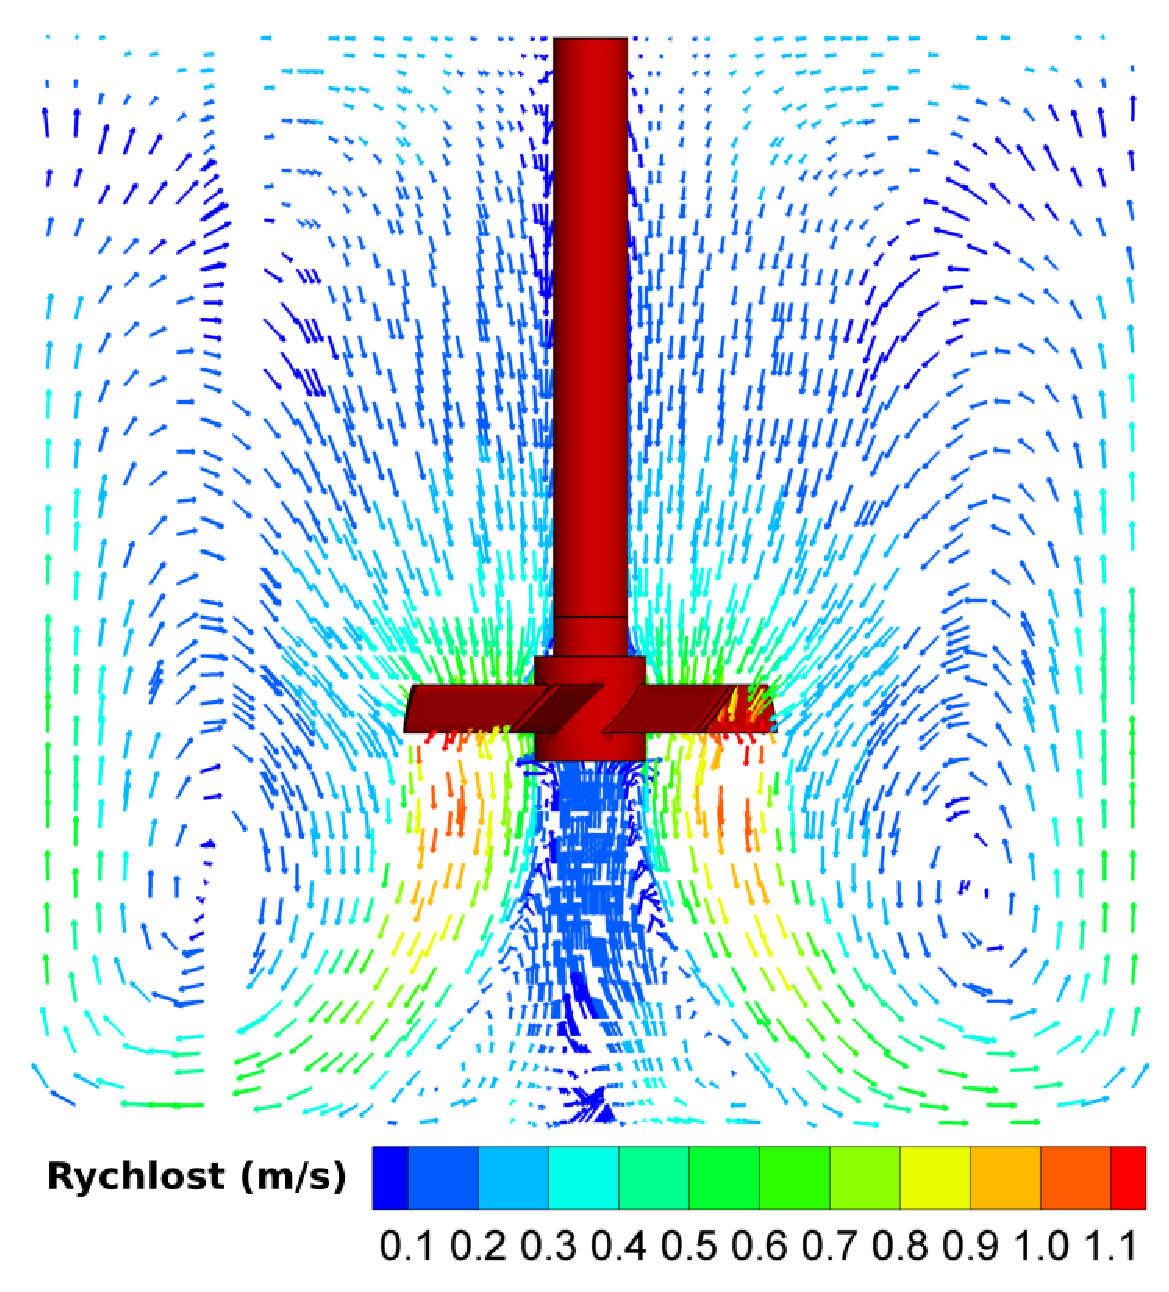
\includegraphics[scale=0.38]{Results/Velocity/keps-std.eps}}  
  \qquad 
  \subfloat[RNG \keps{}]{\label{fig:rng}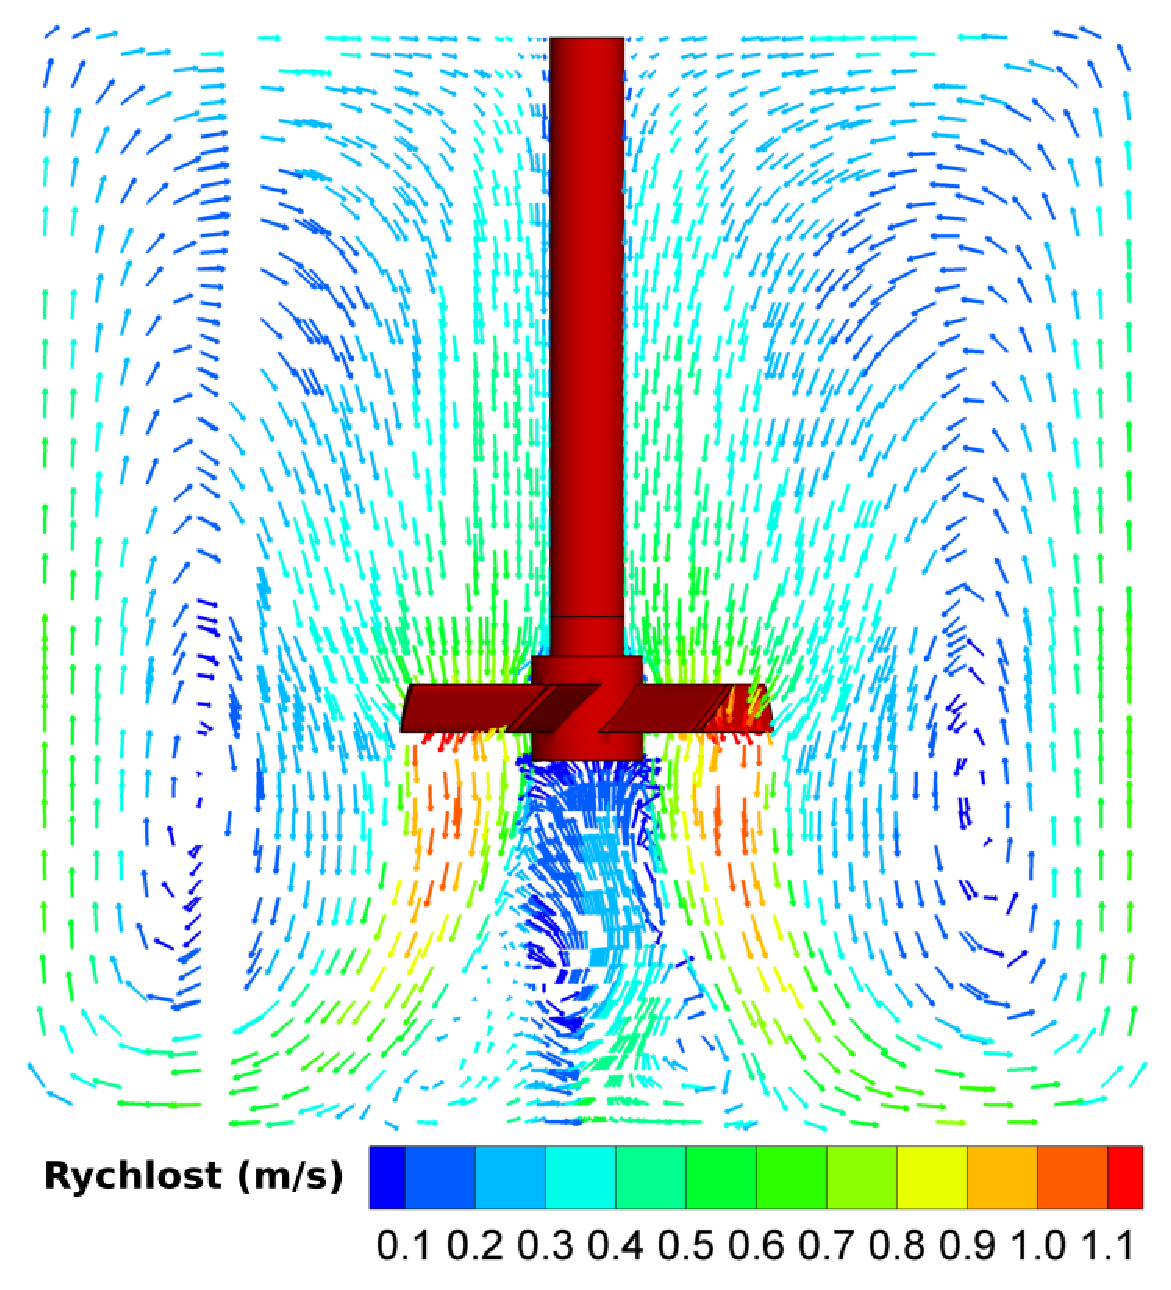
\includegraphics[scale=0.38]{Results/Velocity/keps-RNG.eps}}
\end{figure}
\newpage
\begin{figure}[t!]
  \addtocounter{subfigure}{2}
 \centering
  \subfloat[Realisable \keps{} ]{\label{fig:real}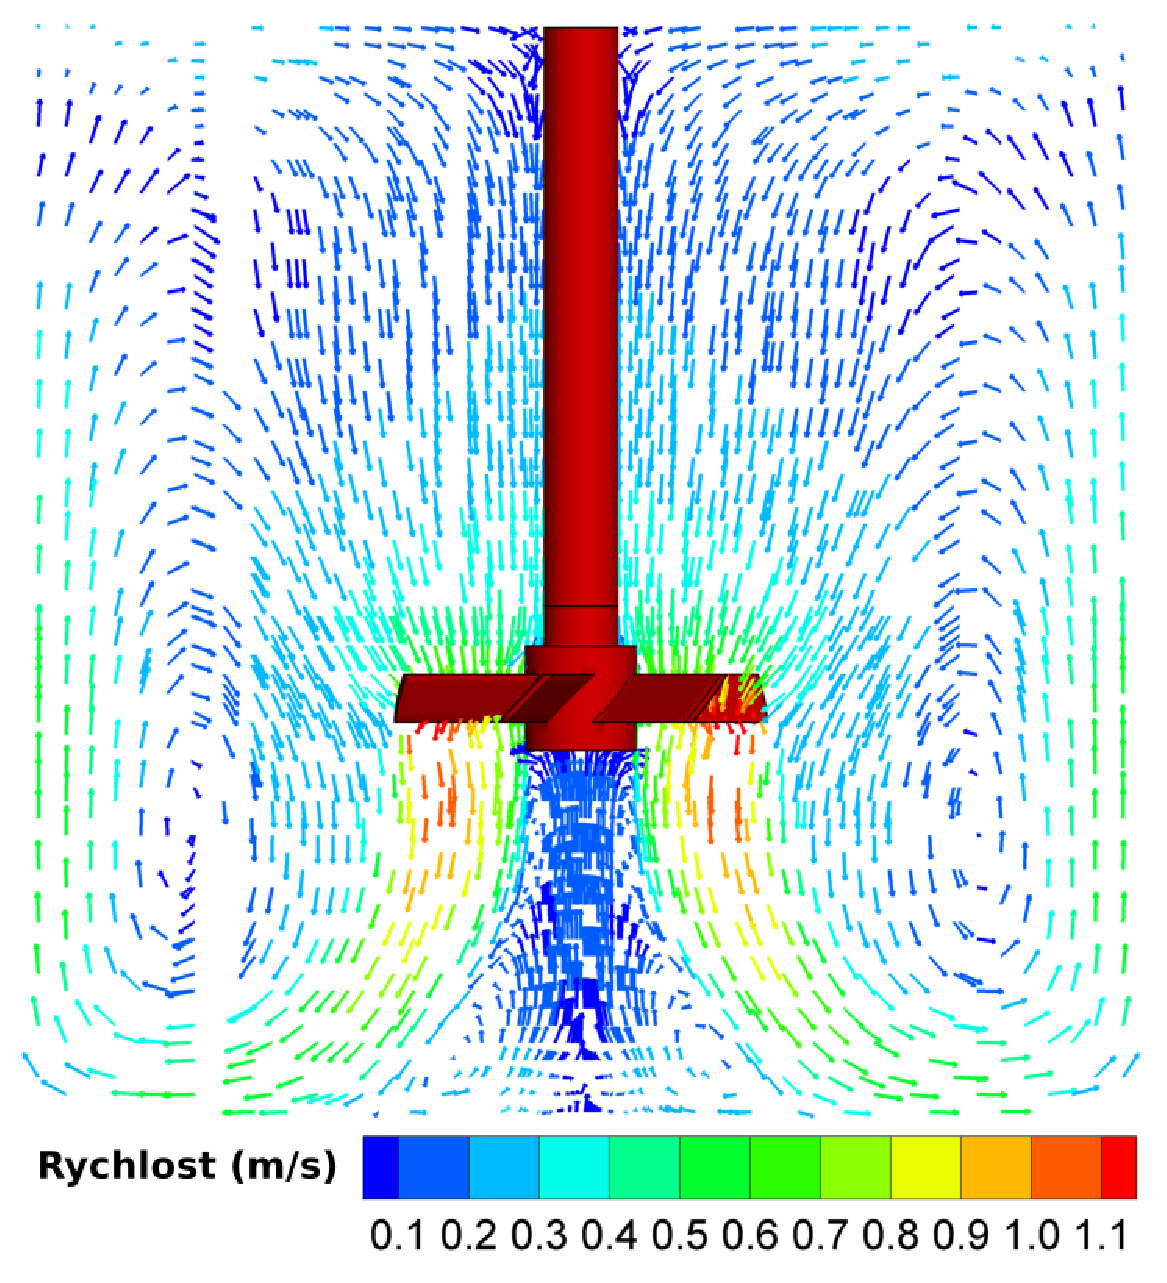
\includegraphics[scale=0.38]{Results/Velocity/keps-real.eps}}
  \qquad
  \subfloat[Standardní RMS]{\label{fig:RMS}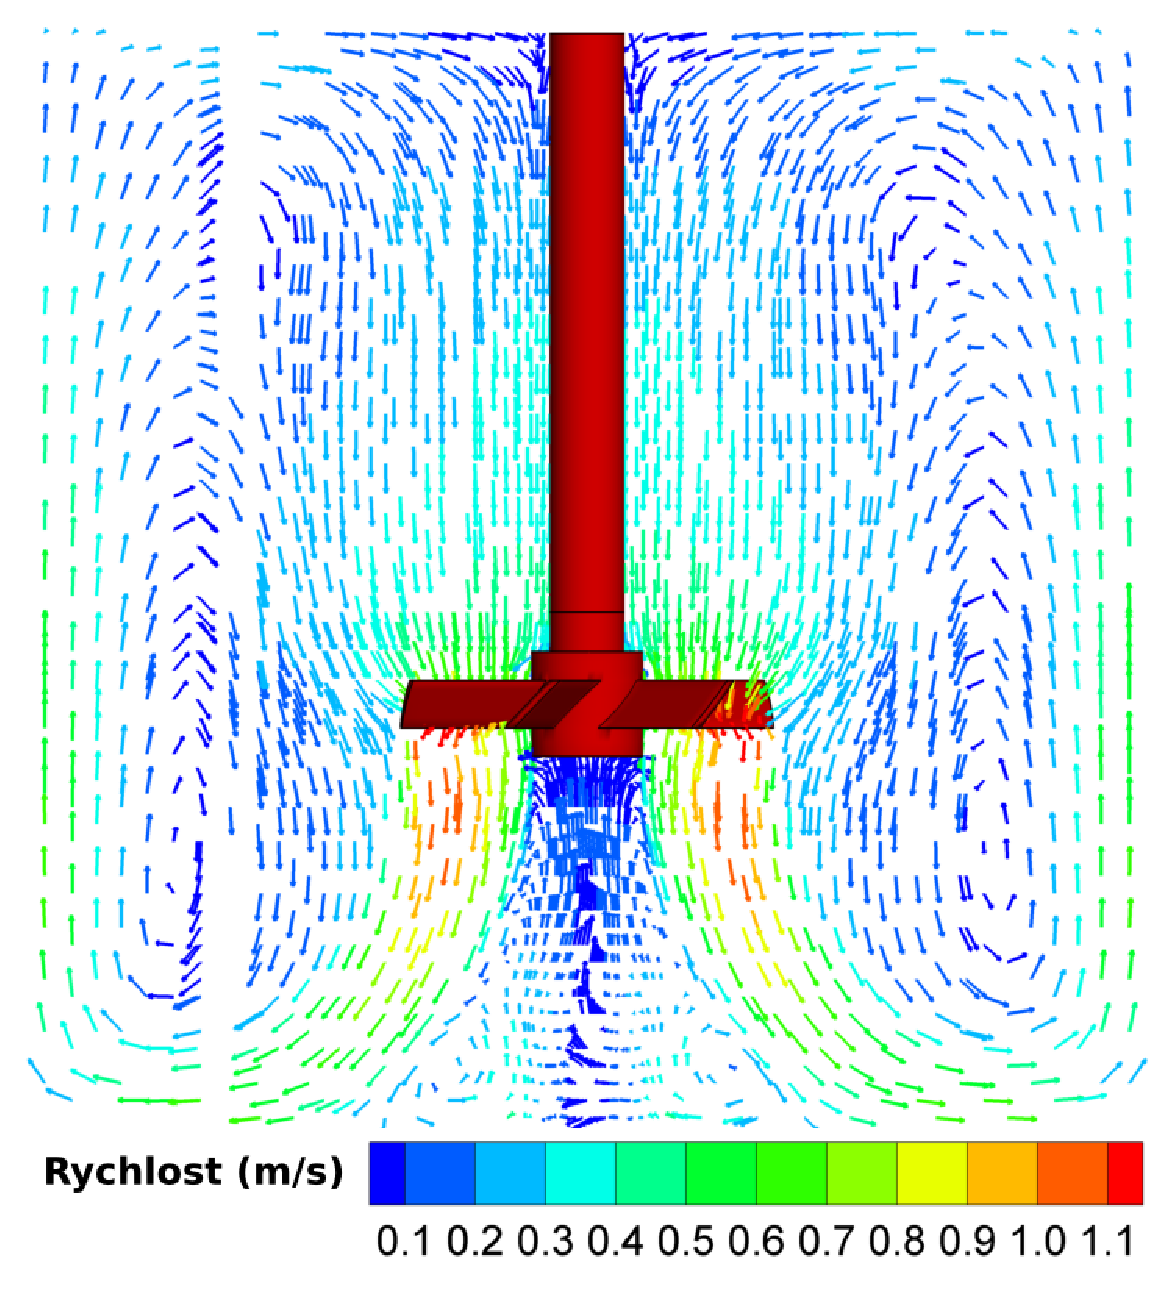
\includegraphics[scale=0.38]{Results/Velocity/RMS.eps}}
  \caption{Vektorové pole rychlosti pro různé turbulentní modely}
  \label{fig:velfield}
\end{figure}

Graf \ref{grf:velfield} zachycuje závislost mezi celkovou rychlostí pohybu kapaliny a vzdáleností ode dna nádoby ($y$) pro jednotlivé turbulentní modely. Konkretní hodnoty pro tento byly získány ve vzdálenosti \SI{0.5}{\centi\meter} podél jedné z narážek nádoby. Z grafu je dobře patrné, že u dna nádrže dochází nárůstu rychlosti tekutiny vlivem působení primární cirkulační smyčky.

\begin{grf}[h!]
 \centering
  \includegraphics[scale=0.45]{Results/Velocity/velField.eps}
  \caption{Průběh velikosti rychlosti tekutiny v nádobě}
  \label{grf:velfield}
\end{grf}

\section{Srovnání modelů pro koeficient odporu}
Jednotlivé modely pro koeficient odporu uvedené v podkapitole \ref{kap:cd} byly porovnány během nestacionární simulace systému obsahující jako vsádku \volproc{5} kuliček z PVC a kapalinu \pvpP. Rychlost otáčení míchadla byla v tomto případě opět nastavena na \SI{7}{\per\second}.

Obr. \ref{fig:cd2} zobrazuje kontury objemového zlomku pevné fáze v~řezu míchací nádobou pro vybrané korelace koeficientu odporu. Tyto údaje byly získány v~času simulace \SI{2}{\second}. 
\begin{figure}[h!]
 \centering

  \subfloat[Schiller-Naumann]{\label{fig:neu2}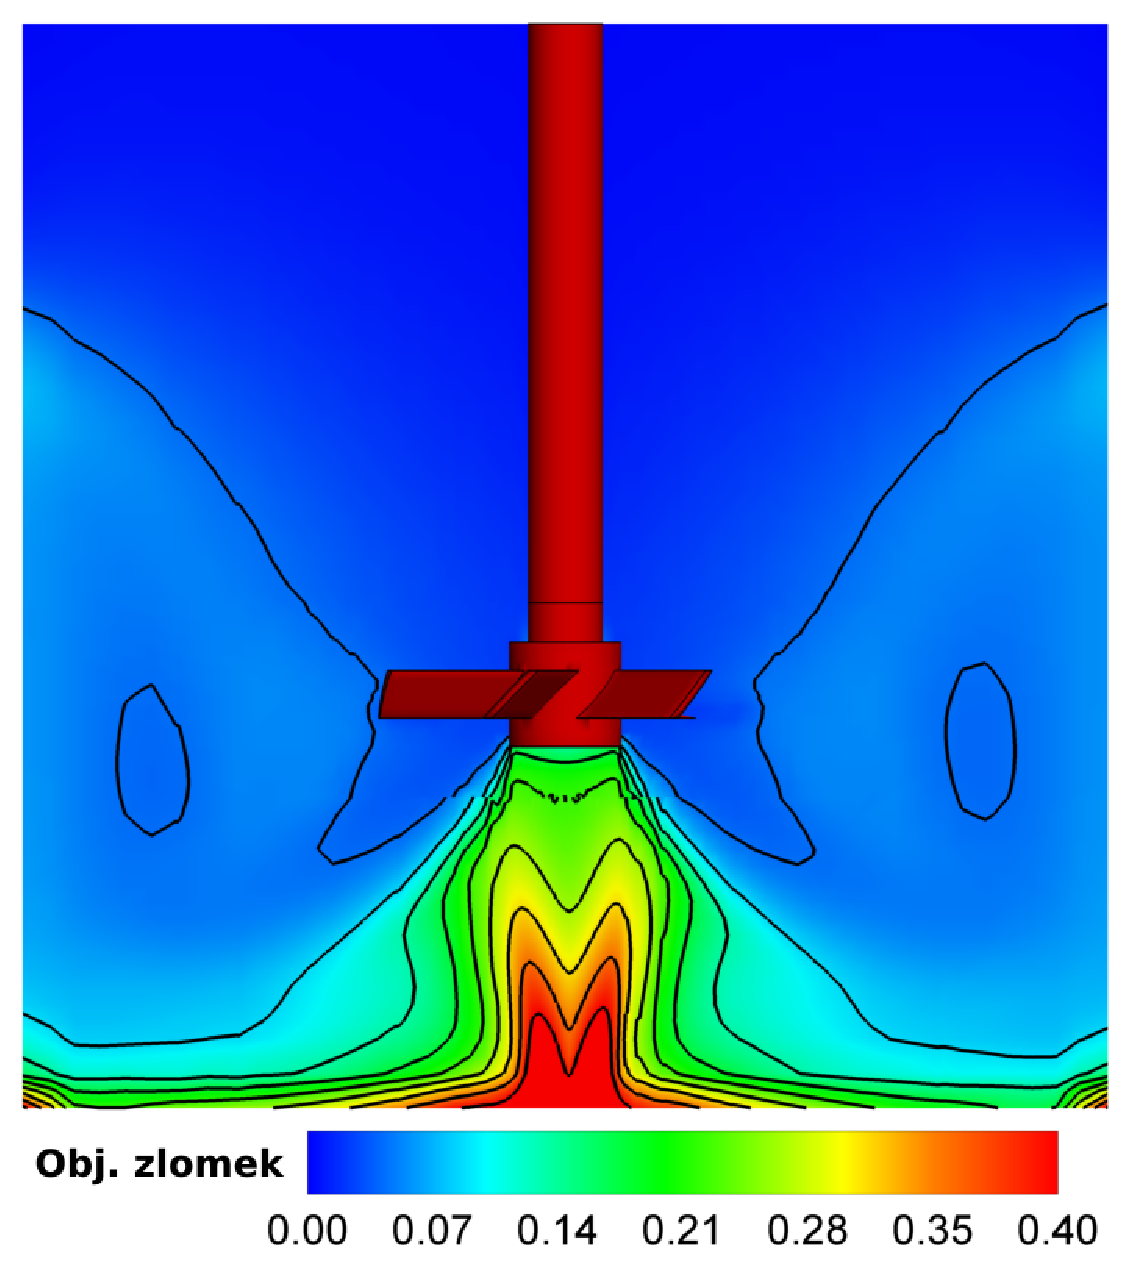
\includegraphics[scale=0.38]{Results/CDComp/neu-2s.eps}}  
  \qquad             
  \subfloat[{Brucato}]{\label{fig:bru2}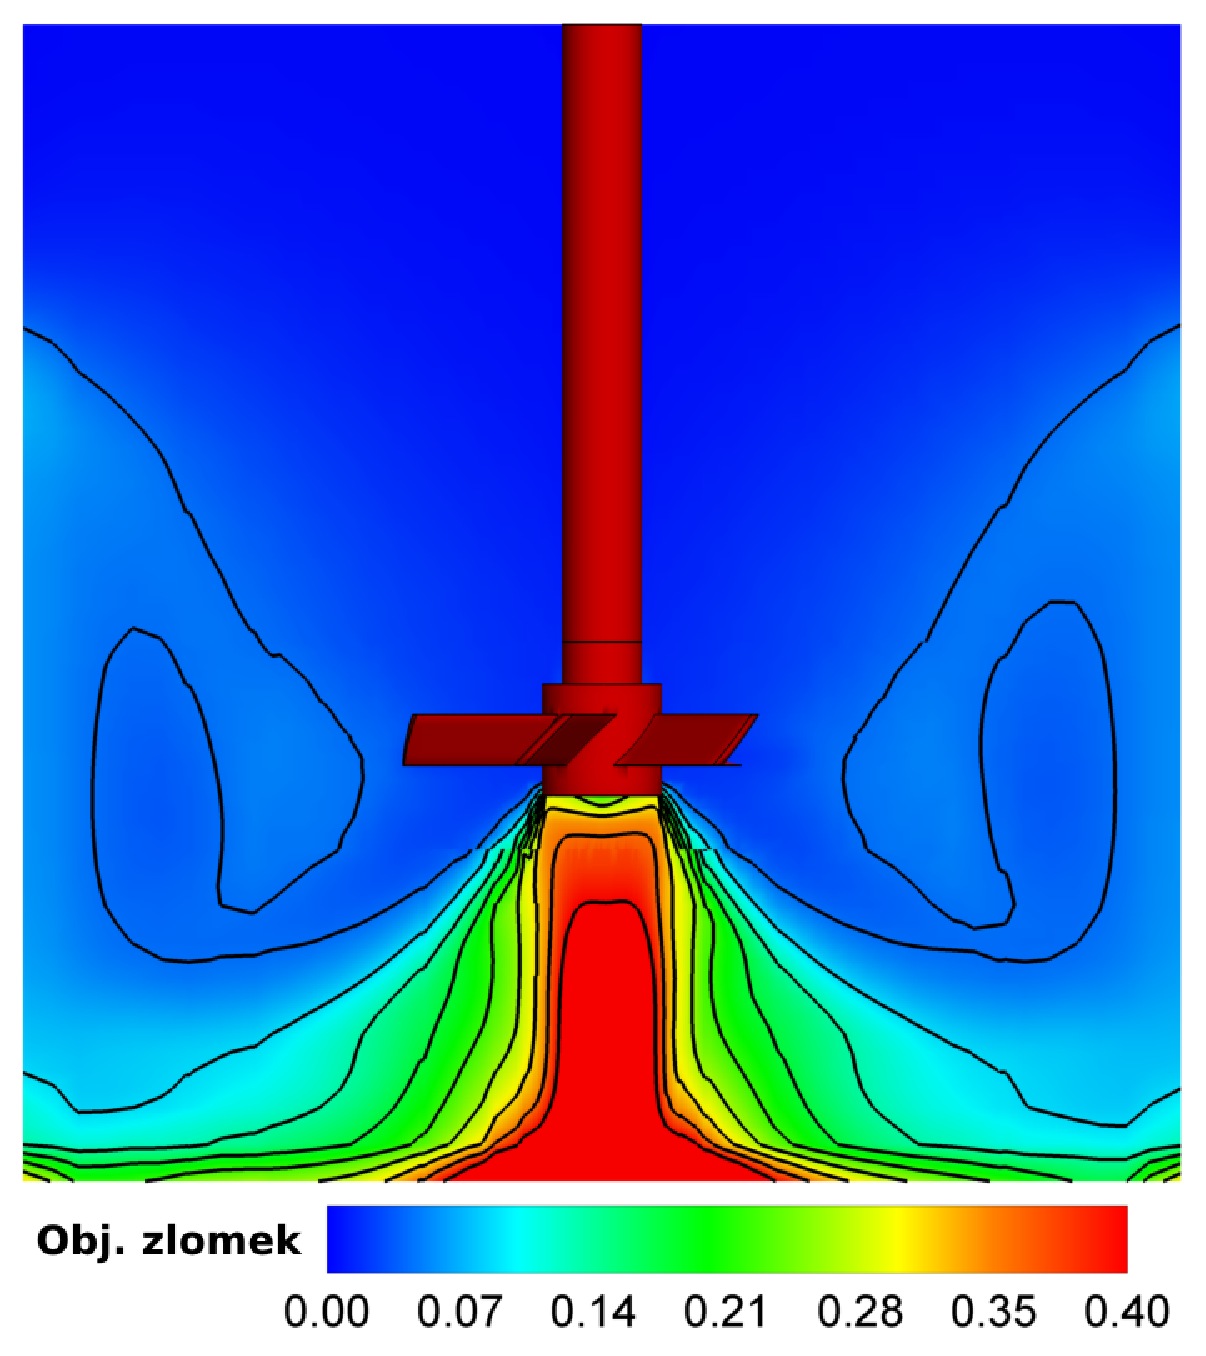
\includegraphics[scale=0.357]{Results/CDComp/bru-2s.eps}}
%\end{figure}
%\newpage
%\begin{figure}[t!]
	%\centering{}
  %\addtocounter{subfigure}{2}
  \\
  \subfloat[{Pinelli}]{\label{fig:pin2}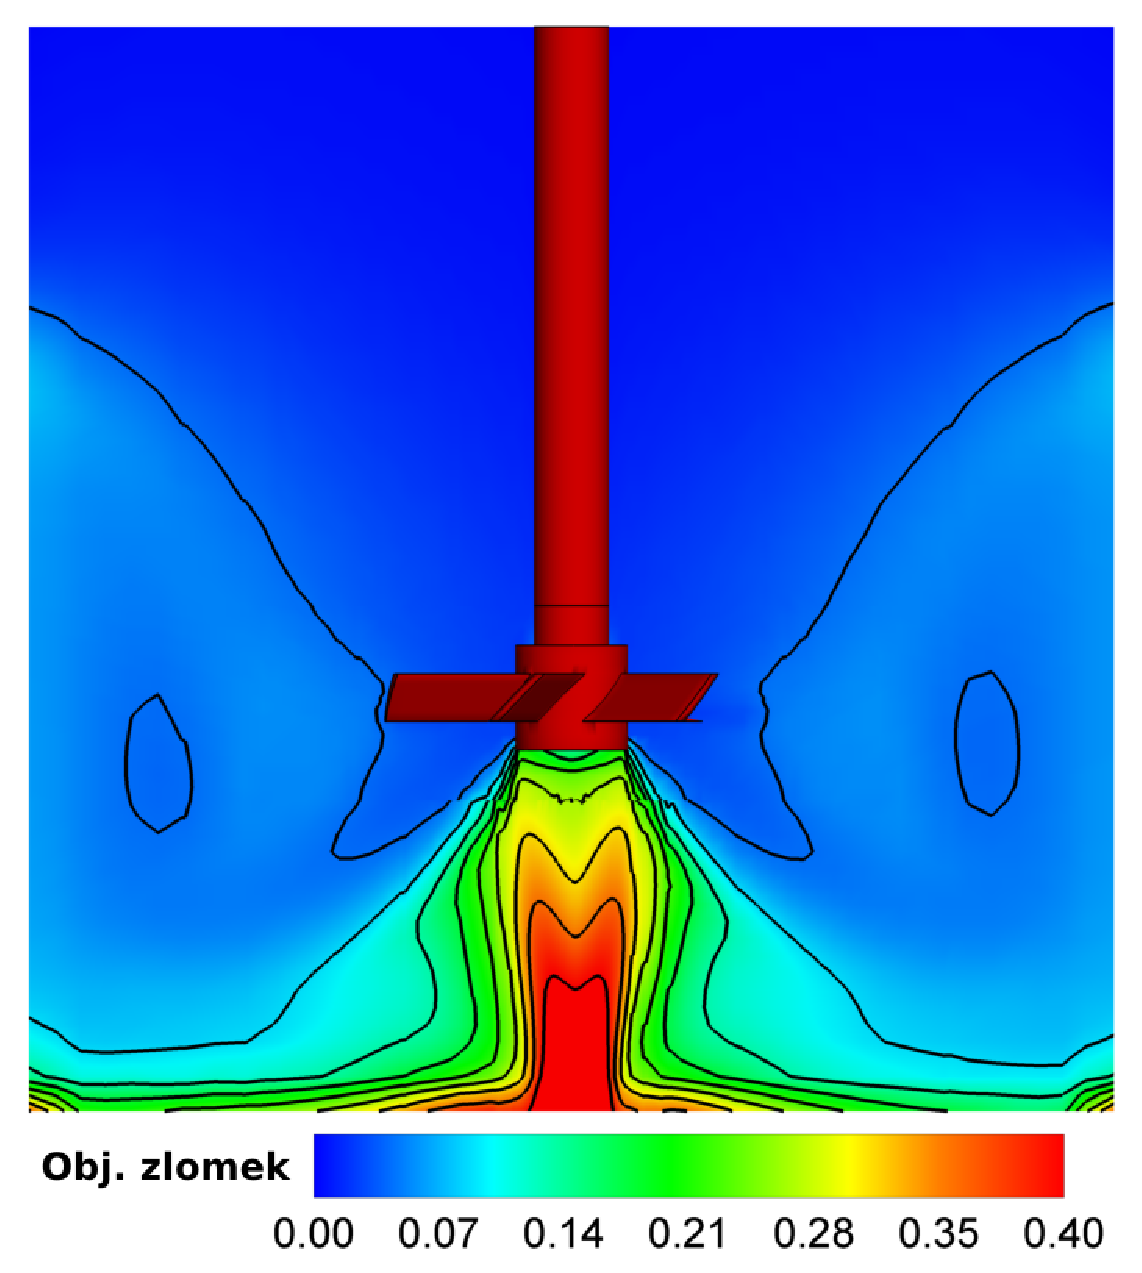
\includegraphics[scale=0.38]{Results/CDComp/pin-2s.eps}}
  \qquad
  \subfloat[{Khopkar}]{\label{fig:kho2}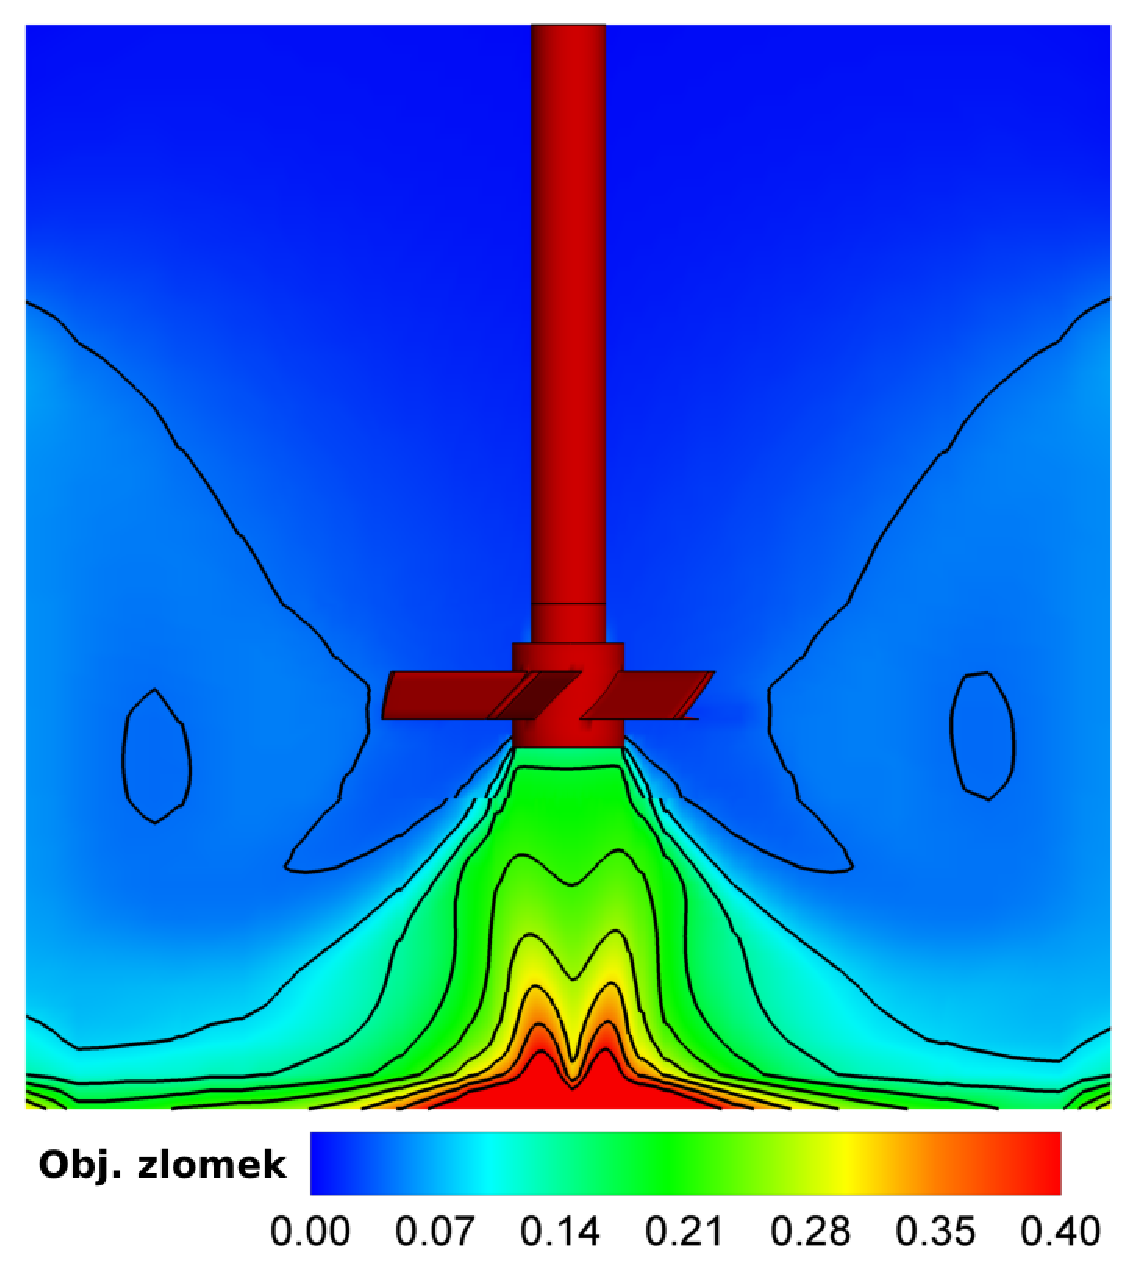
\includegraphics[scale=0.38]{Results/CDComp/kho-2s.eps}}
  \caption{Objemový zlomek pevné fáze v~čase \SI{2}{\second}}
  \label{fig:cd2}
\end{figure}
\newpage
\noindent Z~obrázků je dobře patrné, že přímo pod míchadlem je největší koncentrace pevné fáze vlivem sekundárních cirkulačních smyček, což se podařilo pozorovat i během experimentálního měření.

Série obrázků \ref{fig:cd7} zachycuje objemový zlomek pevné fáze v~řezu nádobou, avšak v čase simulace \SI{7}{\second}. Částice z PVC jsou již značně rozptýleny, ale stále se pod míchadlem nachází oblasti s jejich zvýšenou koncentrací. Nicméně v celé nádobě jsou rozdíly v distribuci pevné fáze mezi jednotlivými modely pro koeficient odporu poměrně zanedbatelné.

\begin{figure}[h!]
 \centering
  \subfloat[Schiller-Naumann]{\label{fig:neu7}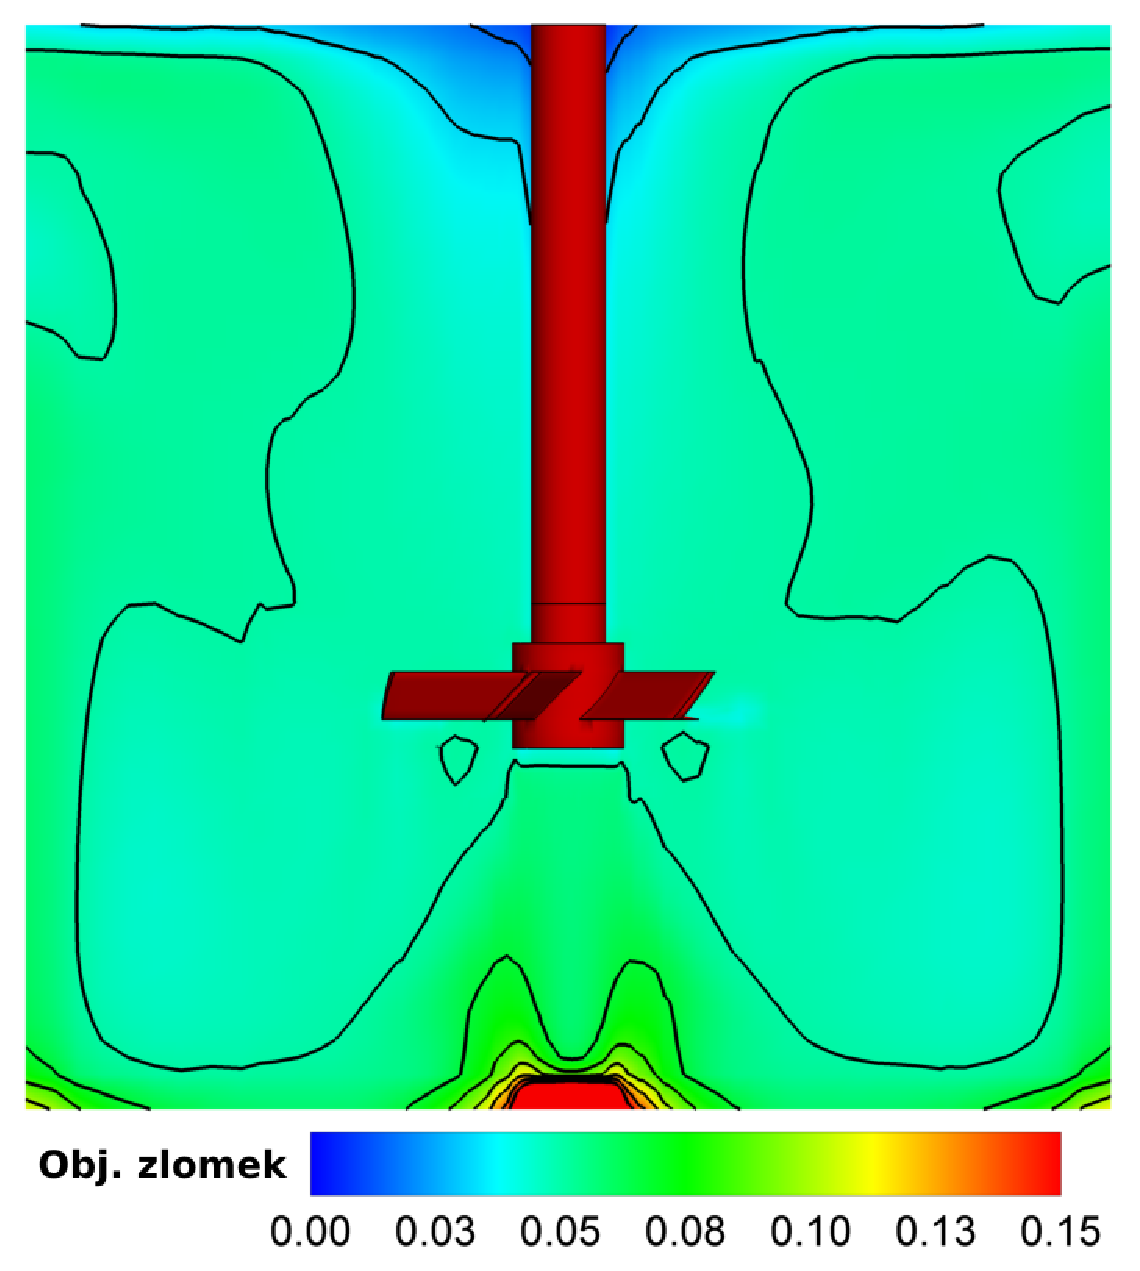
\includegraphics[scale=0.38]{Results/CDComp/neu-7s.eps}}  
  \qquad             
  \subfloat[{Brucato}]{\label{fig:bru7}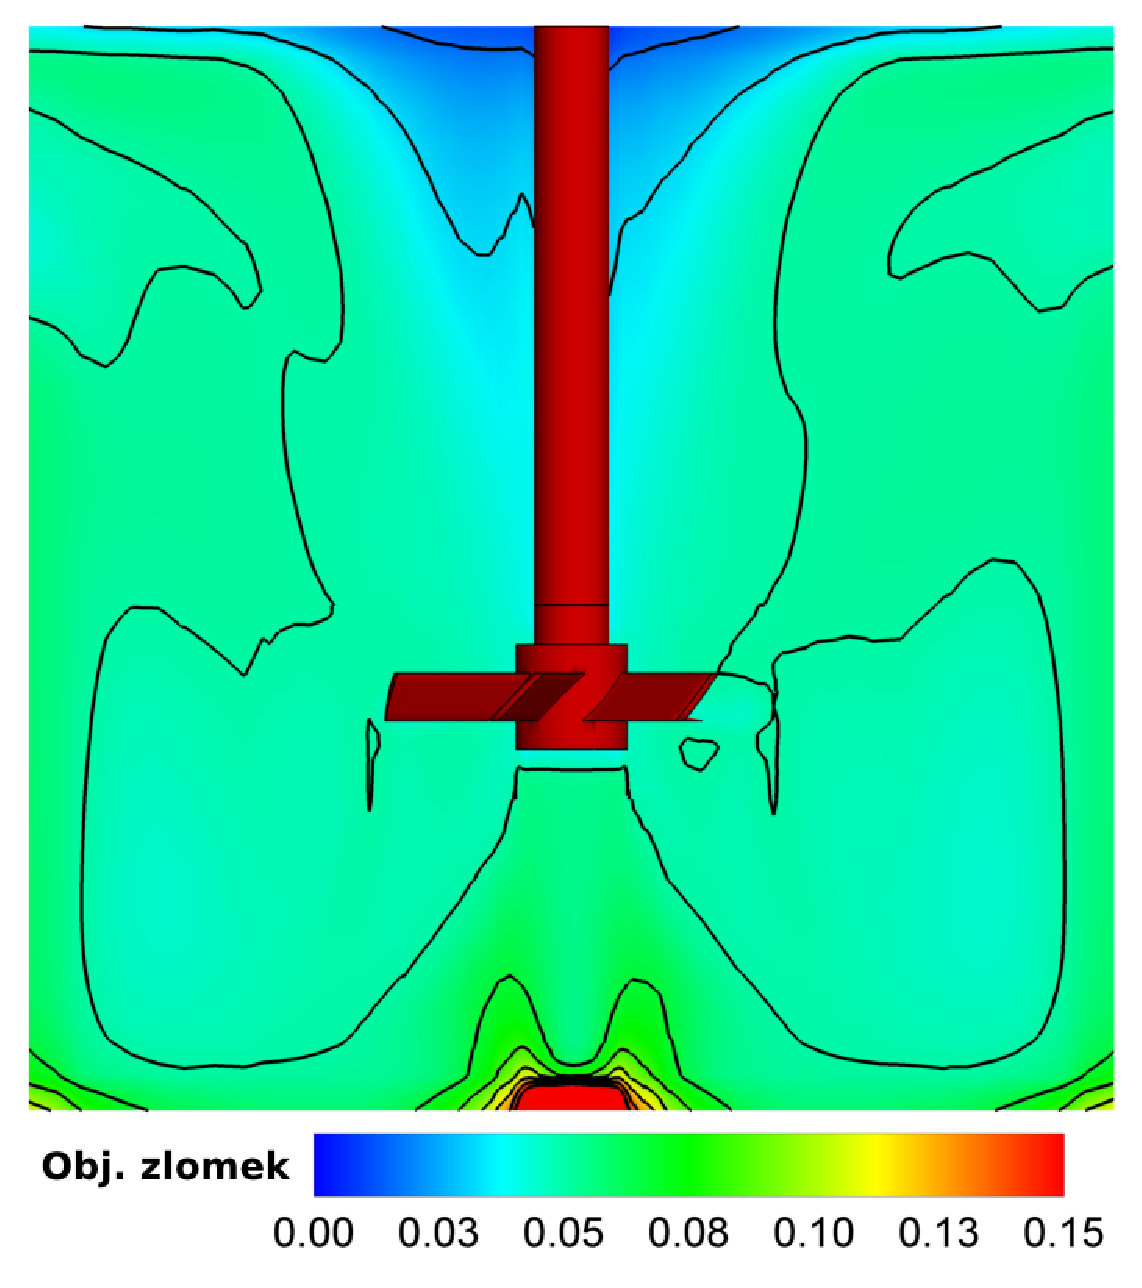
\includegraphics[scale=0.38]{Results/CDComp/bru-7s.eps}}
%\end{figure}
%\newpage
%\begin{figure}[t!]
	 %\centering{}
	 \\
  \subfloat[{Pinelli}]{\label{fig:pin7}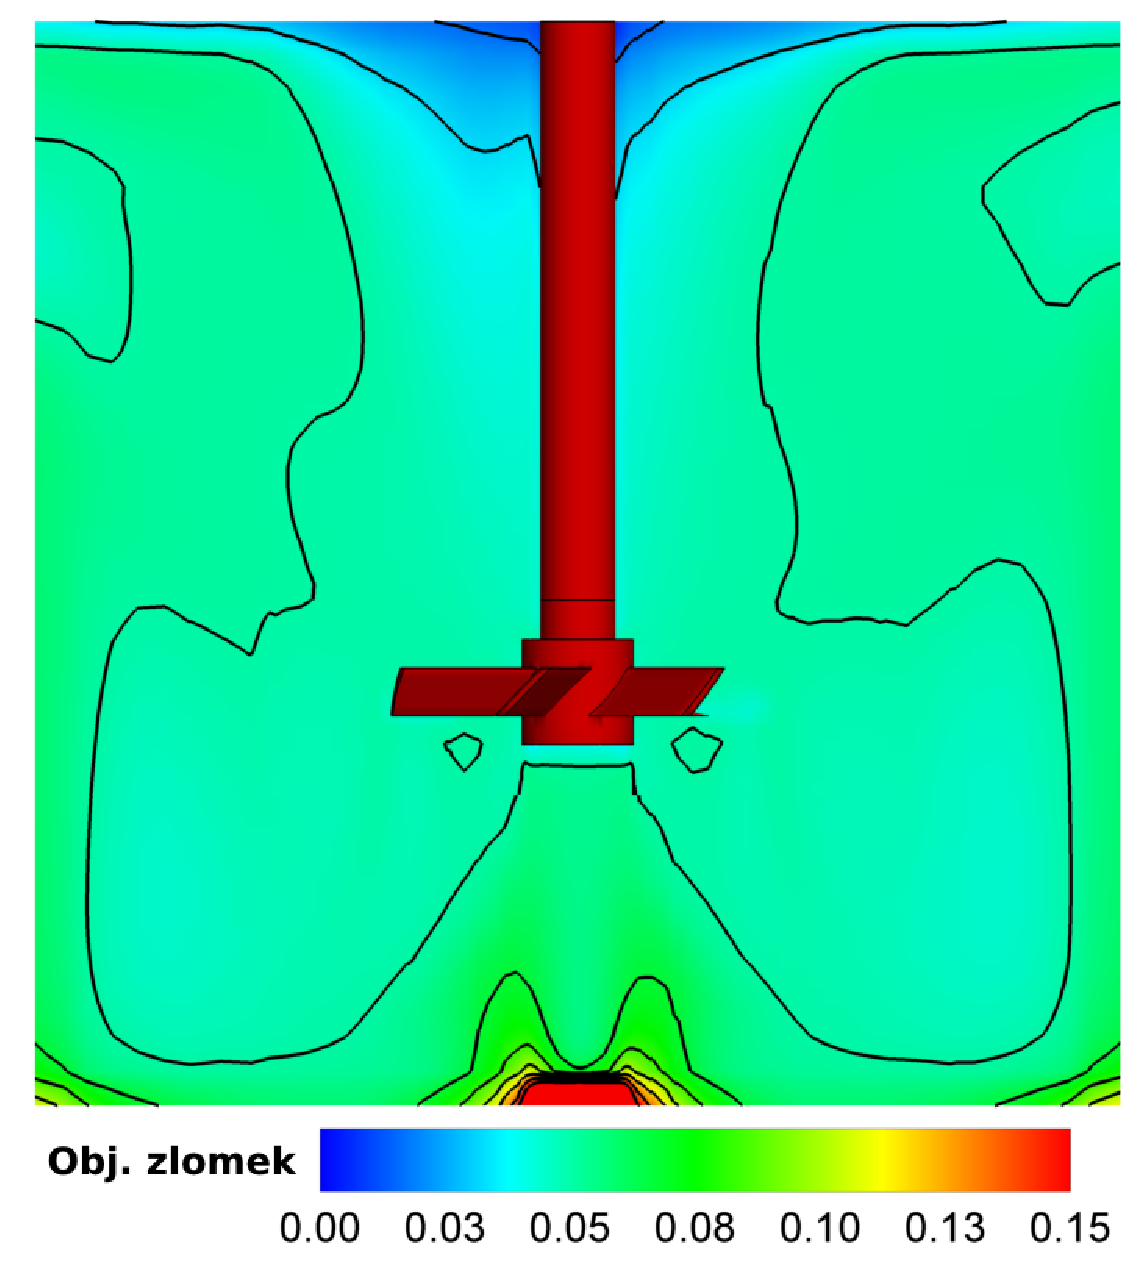
\includegraphics[scale=0.38]{Results/CDComp/pin-7s.eps}}
  \qquad
  \subfloat[{Khopkar}]{\label{fig:kho7}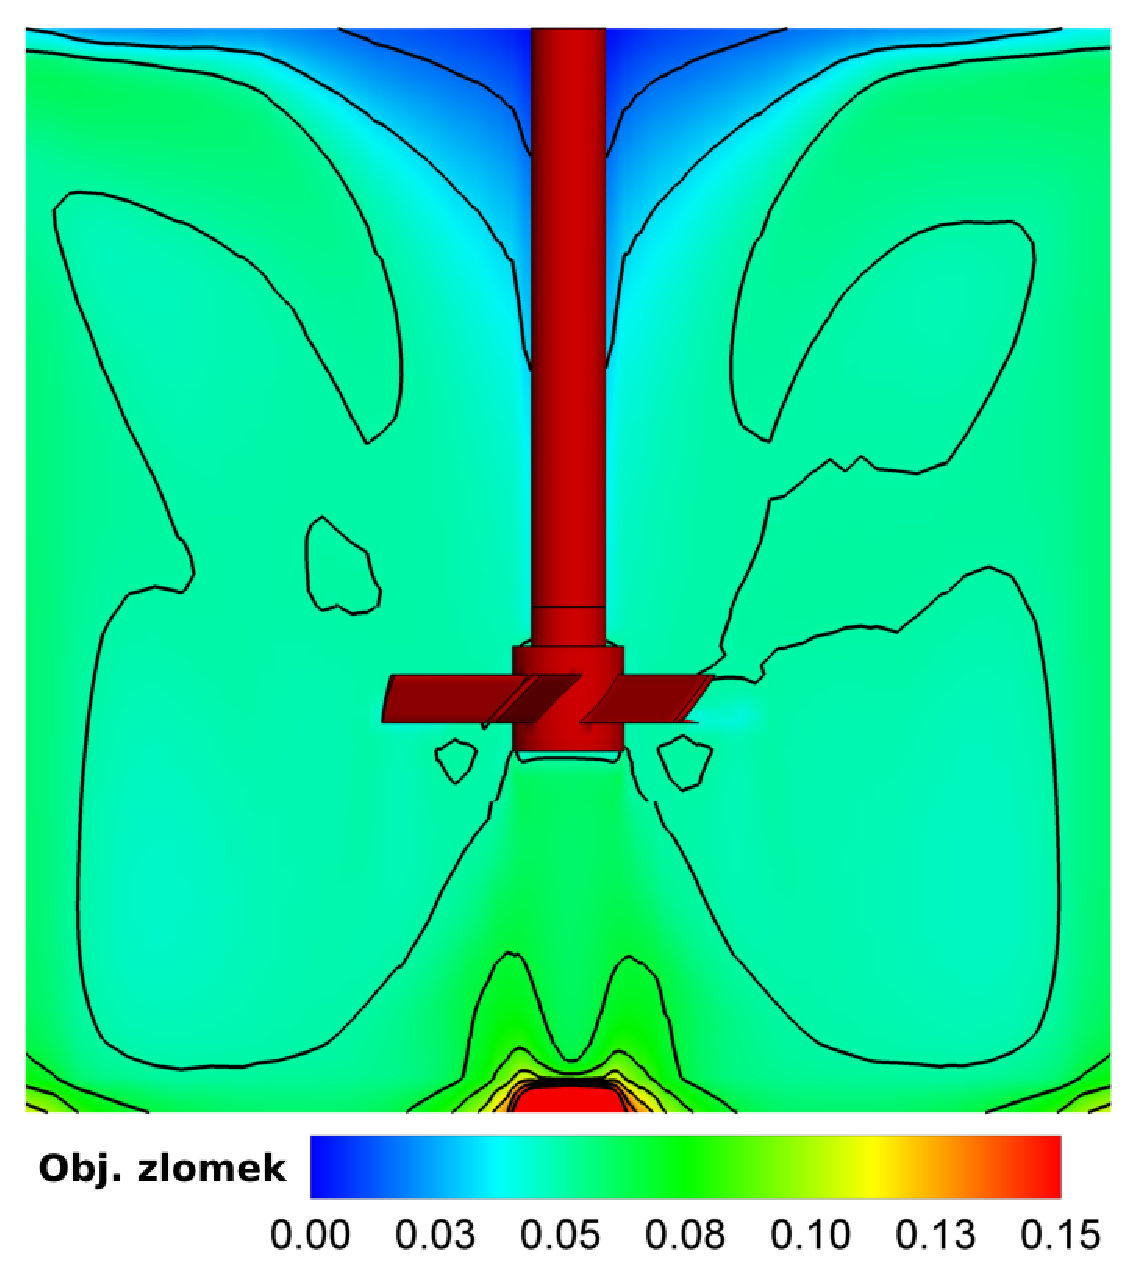
\includegraphics[scale=0.38]{Results/CDComp/kho-7s.eps}}
  \caption{Objemový zlomek pevné fáze v~čase \SI{7}{\second}}
  \label{fig:cd7}
\end{figure}
\newpage
\vspace{-5mm}
Dále jsou zde uvedeny grafické závislosti objemového zlomku pevné fáze na vzdálenosti ode dna nádoby. Z grafu \ref{fig:vol-2} lze vidět, že s~rostoucí vzdáleností se koncentrace pevné fáze postupně snižuje. Avšak grafická závislosti nemá monotonní průběh, přičemž dochází k~tvorbě esovitého koncentračního profilu. Model koeficientu odporu navržený Brucatem předpovídá nižší koncentraci pevné fáze ve vyšší vzdálenosti ode dna než zbylé tři modely. V~čase \SI{7}{\second} kuličky z~PVC již dosáhly značného vznosu a rozdíly mezi jednotlivými korelace pro koeficient odporu se začínaly vytrácet (viz. graf \ref{fig:vol-7}).
\begin{grf}[h!]
 \centering
  \subfloat[v~čase \SI{2}{\second}]{\label{fig:vol-2}\includegraphics[scale=0.39]{Results/CDComp/vol-2s.eps}} 
  \\ 
  \subfloat[v~čase \SI{7}{\second}]{\label{fig:vol-7}\includegraphics[scale=0.39]{Results/CDComp/vol-7s.eps}}
  \caption{Průběh objemového zlomku pevné fáze}
  \label{fig:vol}
\end{grf}
\newpage

Poslední skupina grafů \ref{fig:cd} zachycuje průběh normalizované hodnoty koeficientu odporu v závislosti na světlé výšce. Tato normalizace vznikla vydělením koeficientu odporu jeho průměrnou hodnotou v celé nádrži. Údaje v těchto grafech byly stanoveny podél úsečky v blízkosti radiální narážky.  V~obou případech má  koeficientu odporu podobný průběh pro různé korelace, nicméně v čase \SI{7}{\second} (graf \ref{fig:cd-2}) je zřejmé, že korelace dle Brucata se opět nejznatelněji odlišuje.

\begin{grf}[h!]
 \centering
  \subfloat[v~čase \SI{2}{\second}]{\label{fig:cd-2}\includegraphics[scale=0.40]{Results/CDComp/cd-2s.eps}} 
  \\ 
  \subfloat[v~čase \SI{7}{\second}]{\label{fig:cd-7}\includegraphics[scale=0.40]{Results/CDComp/cd-7s.eps}}
  \caption{Průběh hodnoty koeficientu odporu}
  \label{fig:cd}
\end{grf}
\newpage

\section{Výška vznosu pevné fáze}
Výška suspenzního mraku byla stanovena pro systém tvořený kapalinou \pvpS{} a pevnou fází o koncentraci \volproc{10} při třech různých frekvencí otáčení míchadla. Pro vlastní simulaci byl využit vícefázový přístup Eulerian-Eulerian spolu s Khopkarovým model pro koeficient odporu. Pro potřeby CFD výpočtů \citet{kas08} definovali výšku suspenzního mraku jako vzdálenost mezi dnem nádoby a nejvzdálenějším bodem, který má objemový zlomek zrnité fáze roven průměrné koncentraci v nádrži. Stejný přistup pro učení této výšky byl využit i v následující práci.  

Na obrázku \ref{fig:h-w10-4s-num} je zachycen řez nádobou s konturami objemového zlomku pevné fáze získaný pomocí CFD simulace. Frekvence otáčení míchadla v tomto případě činila \SI{4}{\per\second}. Výška vznosu kuliček z PVC byla, pomocí techniky diskutované výše, stanovena v \SI{24.6}{\centi\meter}. Pro srovnání na obr. \ref{fig:h-w10-4s-exp} je ukázána fotografie pořízená během experimentu. Z ni je dobře patrný vznik rozhraní kapalina-pevná fáze přibližně ve výšce \SI{22}{\centi\meter}, přičemž tato vzdálenost byla stanovena pomocí ocelového metru umístěného od \SI{2}{\centi\meter} nad dnem nádoby.

\begin{figure}[h!]
 \centering
  \subfloat[simulace]{\label{fig:h-w10-4s-num}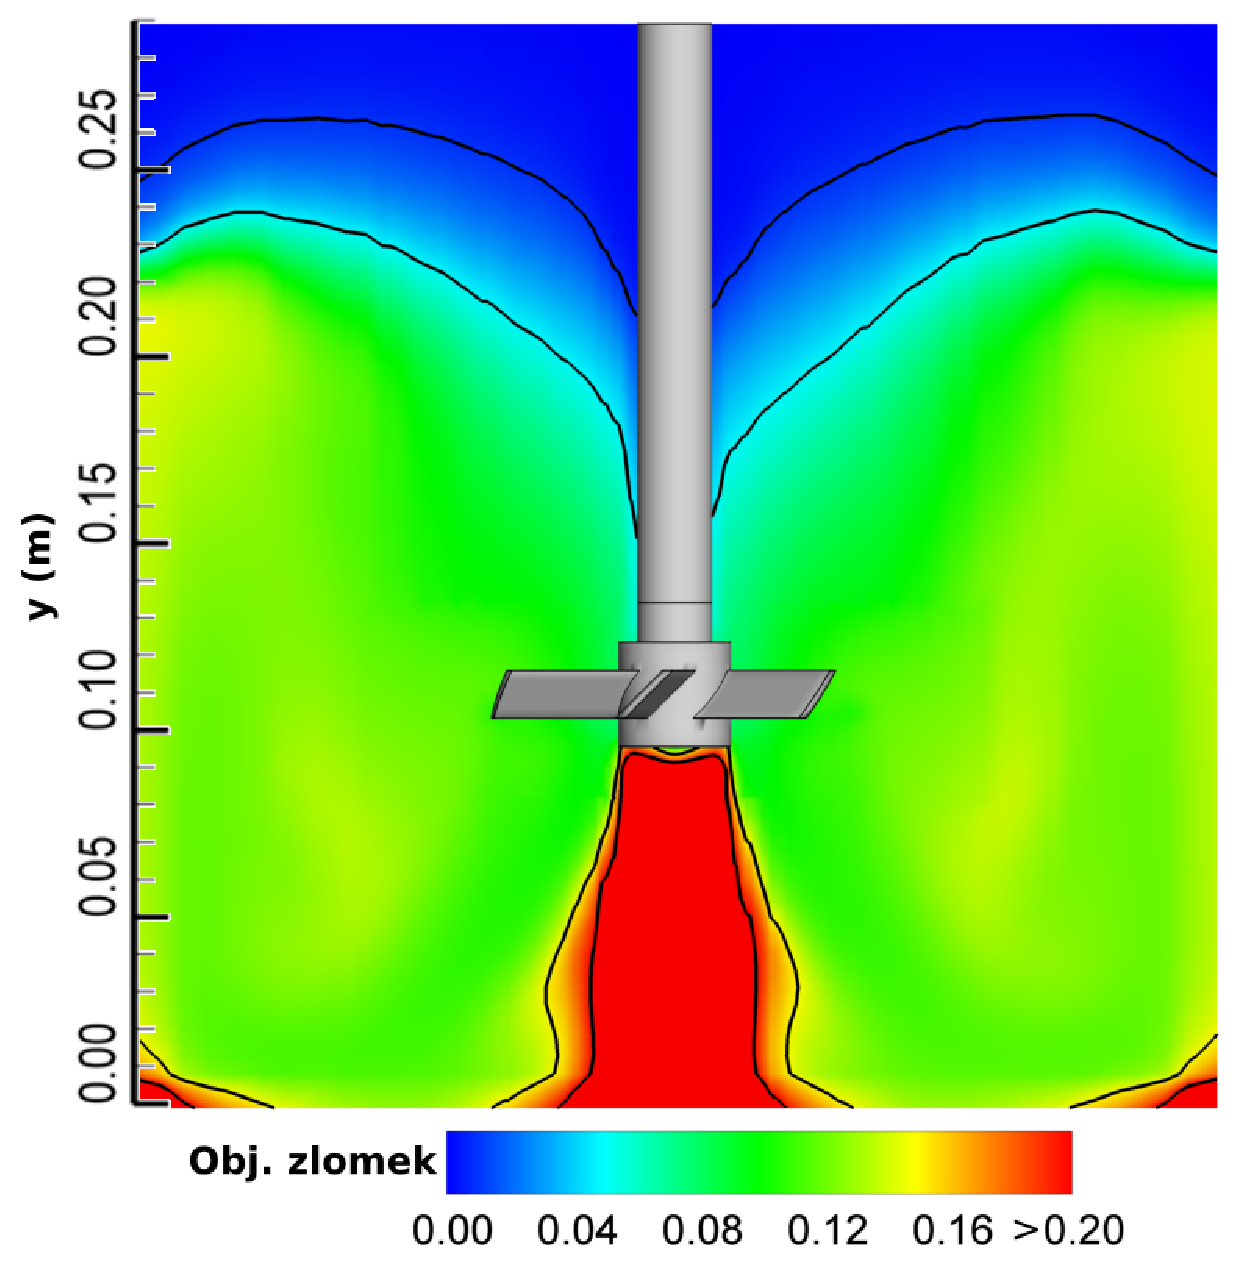
\includegraphics[scale=0.36]{Results/CloudHeight/w10-4s.eps}} 
  \qquad 
  \subfloat[experiment]{\label{fig:h-w10-4s-exp}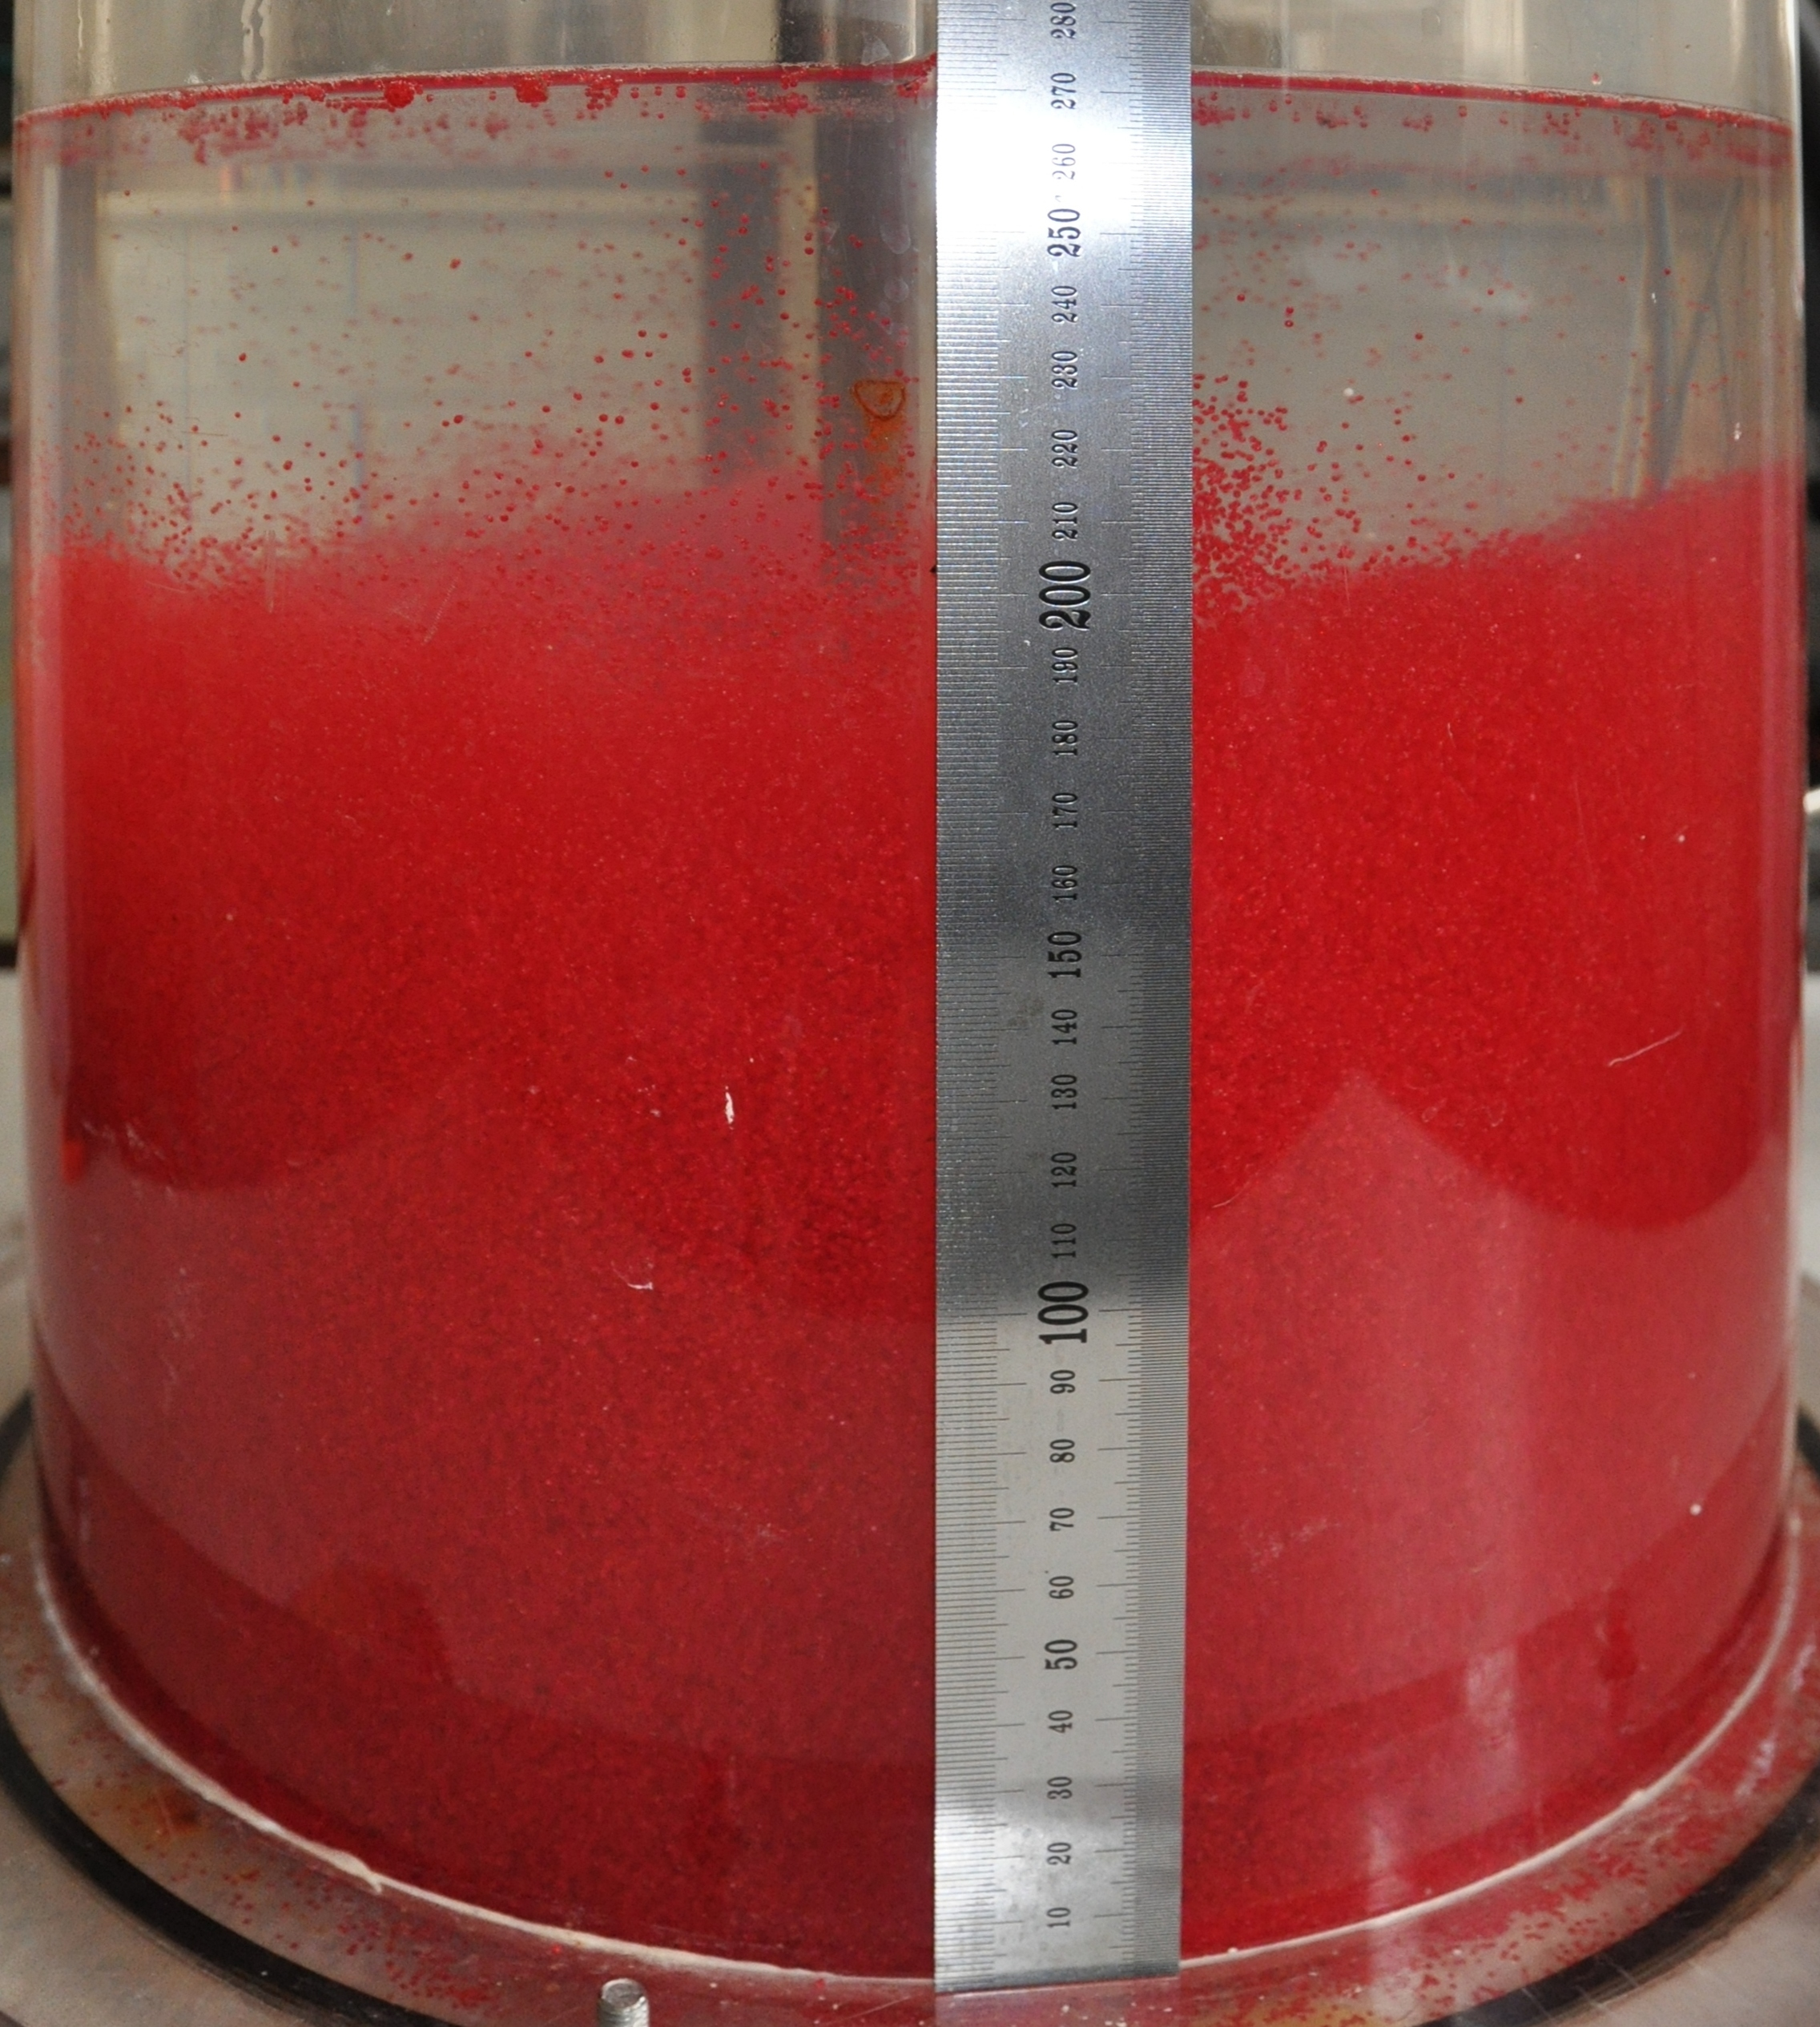
\includegraphics[scale=0.35]{Results/CloudHeight/pvp7-vol10-4s.eps}}
  \caption{Vznos pevné fáze $\kula{N=\SI{4}{\per\second}}$}
  \label{fig:h-w10-4s}
\end{figure}

Vlivem nárůstu rychlosti otáčení míchadla na \SI{5}{\per\second} došlo ke zvýšení výšky suspezního mraku zhruba na \SI{27}{\centi\meter} (viz. obr. \ref{fig:h-w10-5s-exp}). Zmíněný jev byl taktéž pozorován pomocí CFD simulace, což ilustruje řez nádobou \ref{fig:h-w10-5s-num}. Stanovená výška vznosu pevné fáze v tomto případě činila \SI{28.3}{\centi\meter}. 
\newpage

\begin{figure}[t!]
 \centering
  \subfloat[simulace]{\label{fig:h-w10-5s-num}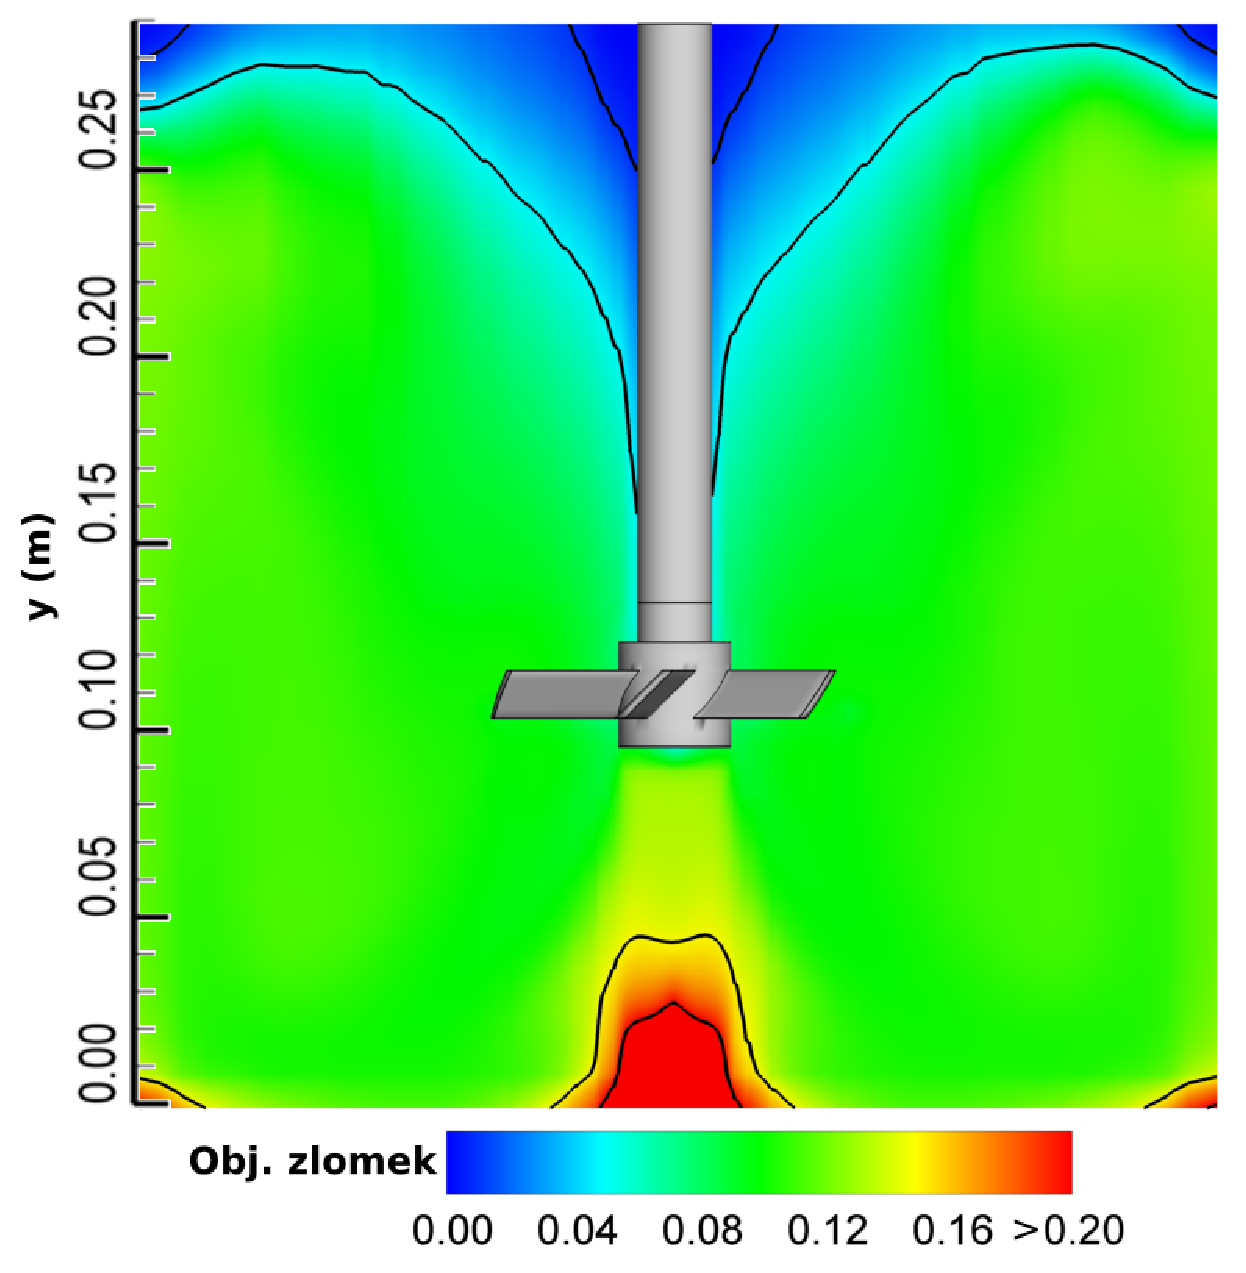
\includegraphics[scale=0.36]{Results/CloudHeight/w10-5s.eps}} 
  \qquad 
  \subfloat[experiment]{\label{fig:h-w10-5s-exp}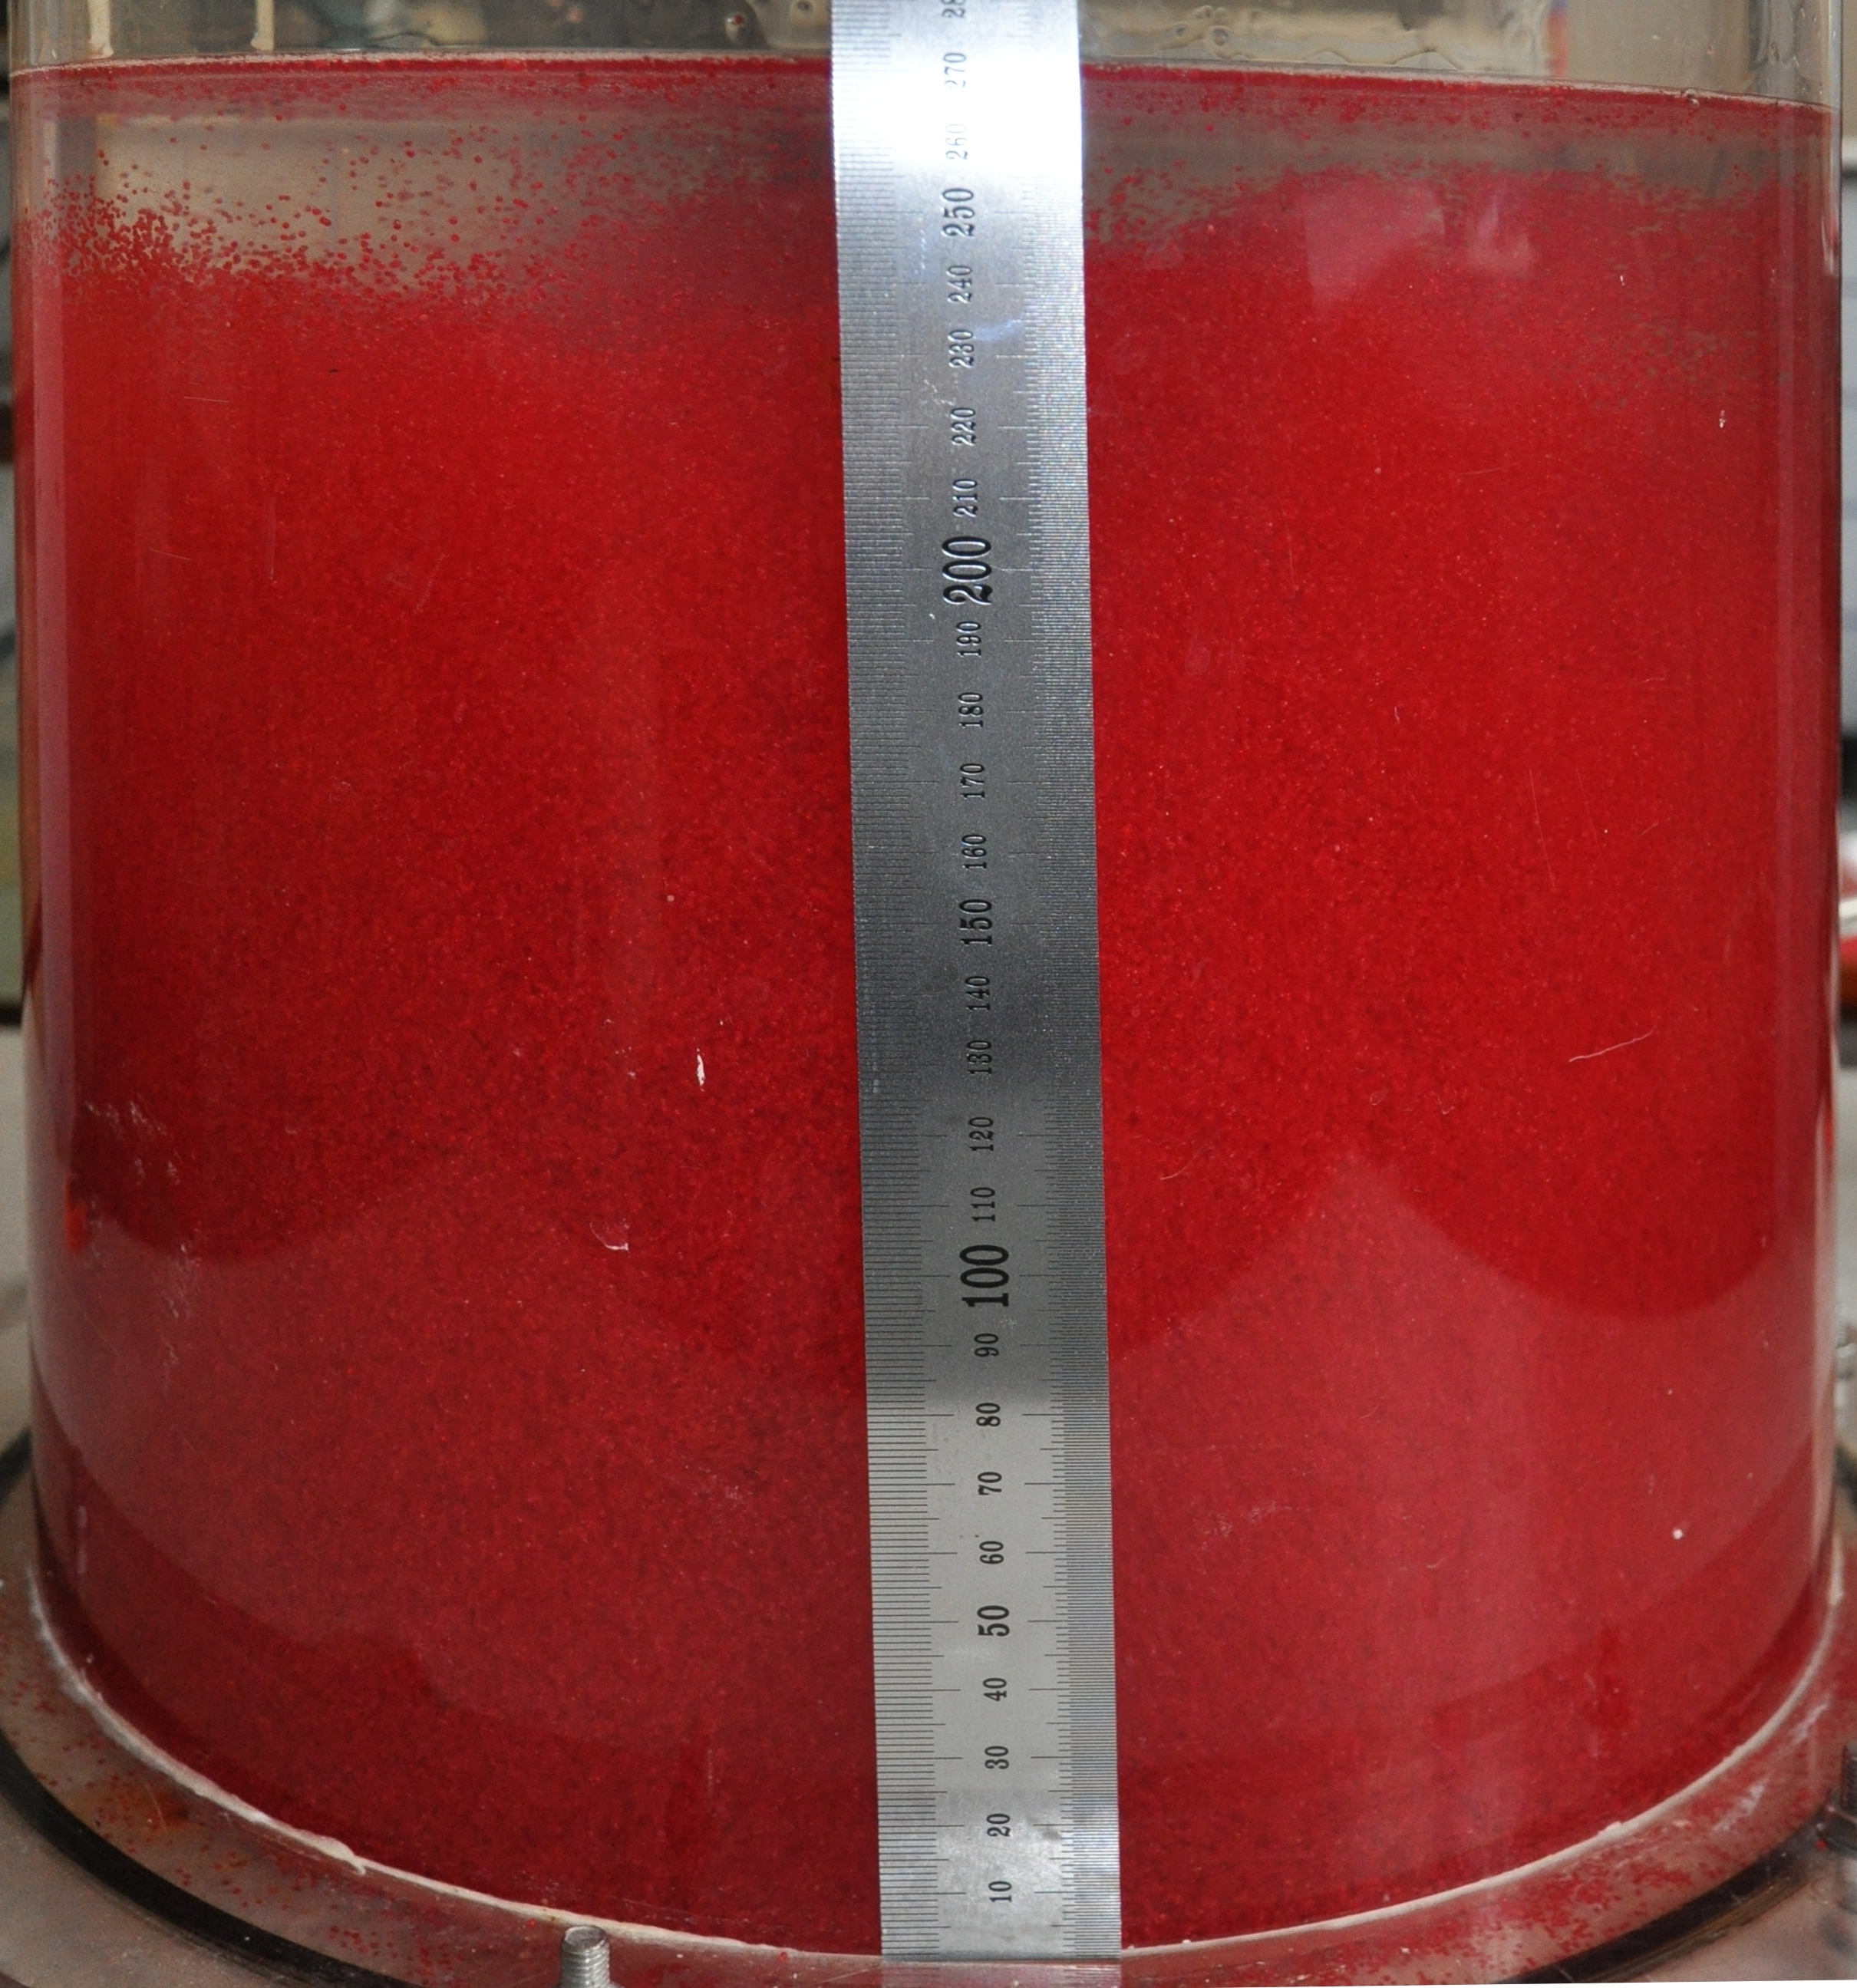
\includegraphics[scale=0.34]{Results/CloudHeight/pvp7-vol10-5s.eps}}
  \caption{Vznos pevné fáze $\kula{N=\SI{5}{\per\second}}$}
  \label{fig:h-w10-5s}
\end{figure}
Poslední skupina obrázků \ref{fig:h-w10-6s} zachycuje stav suspenze při frekvenci otáčení míchadla \SI{6}{\per\second}. Z obrázku \ref{fig:h-w10-6s-exp} lze vidět, že pevná fáze je praticky rozptýlena v celé nádrži, a proto výška suspezního mraku je téměř totožná s výškou plnění nádoby. Obdobný závěr vyplynul i z výsledků ziskaných pomocí CFD simulace (obr. \ref{fig:h-w10-6s-num}), jenž stanovila výšku tohoto mraku na \SI{28.5}{\centi\meter}.

\begin{figure}[h!]
 \centering
  \subfloat[simulace]{\label{fig:h-w10-6s-num}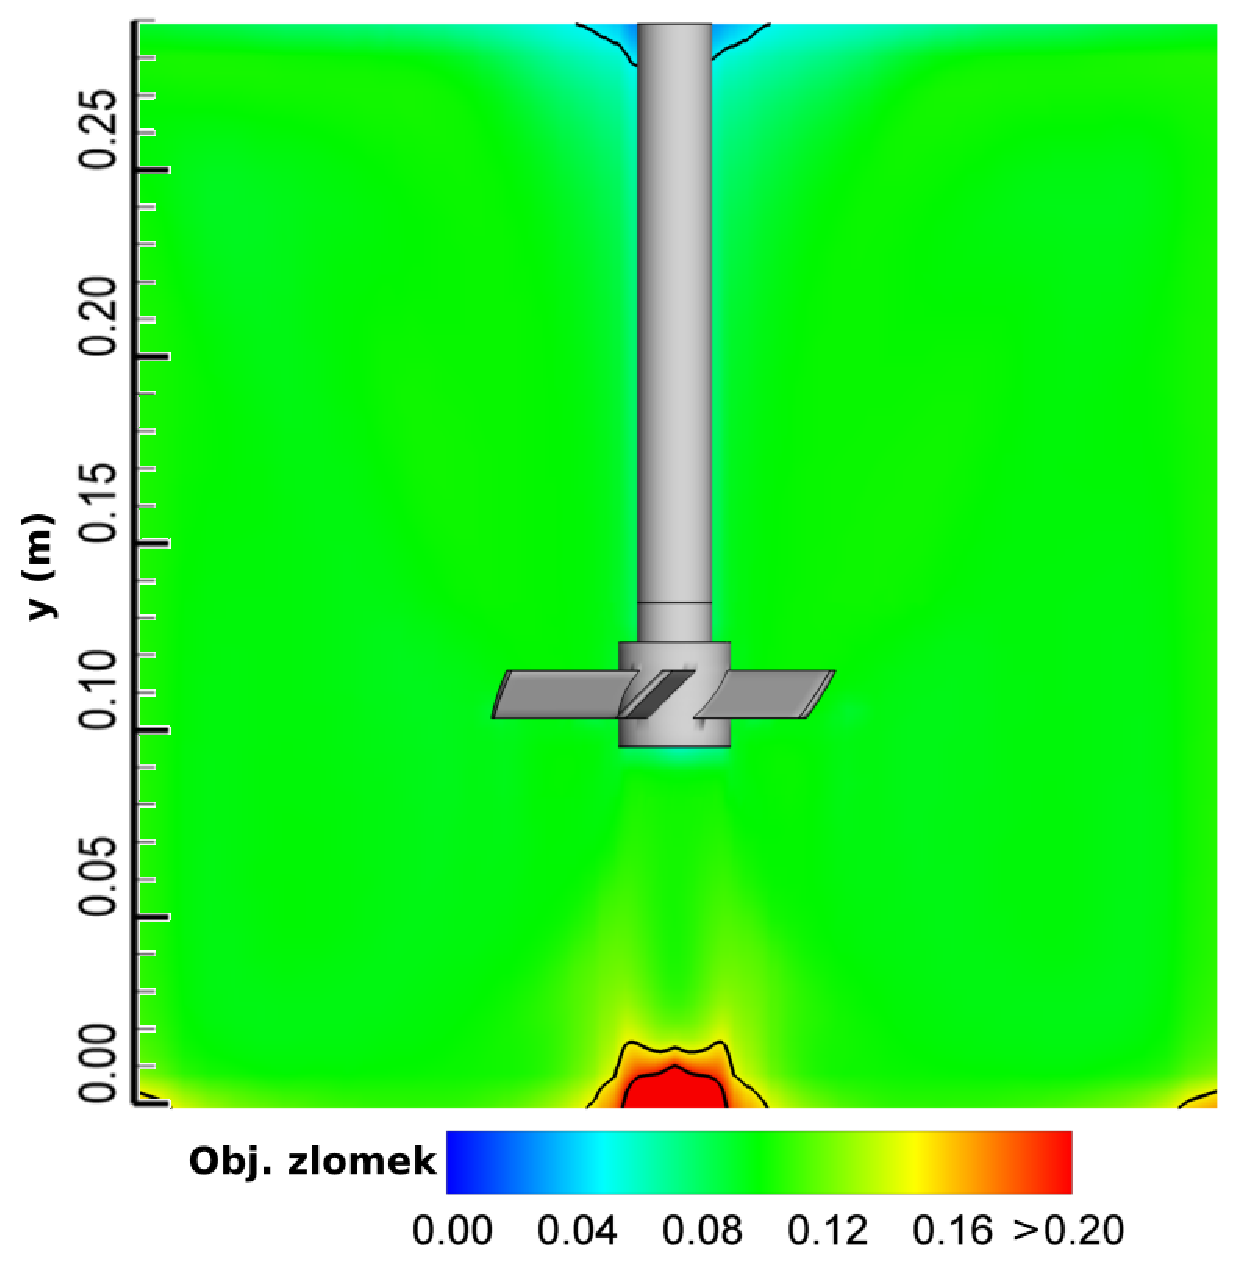
\includegraphics[scale=0.36]{Results/CloudHeight/w10-6s.eps}} 
  \qquad 
  \subfloat[experiment]{\label{fig:h-w10-6s-exp}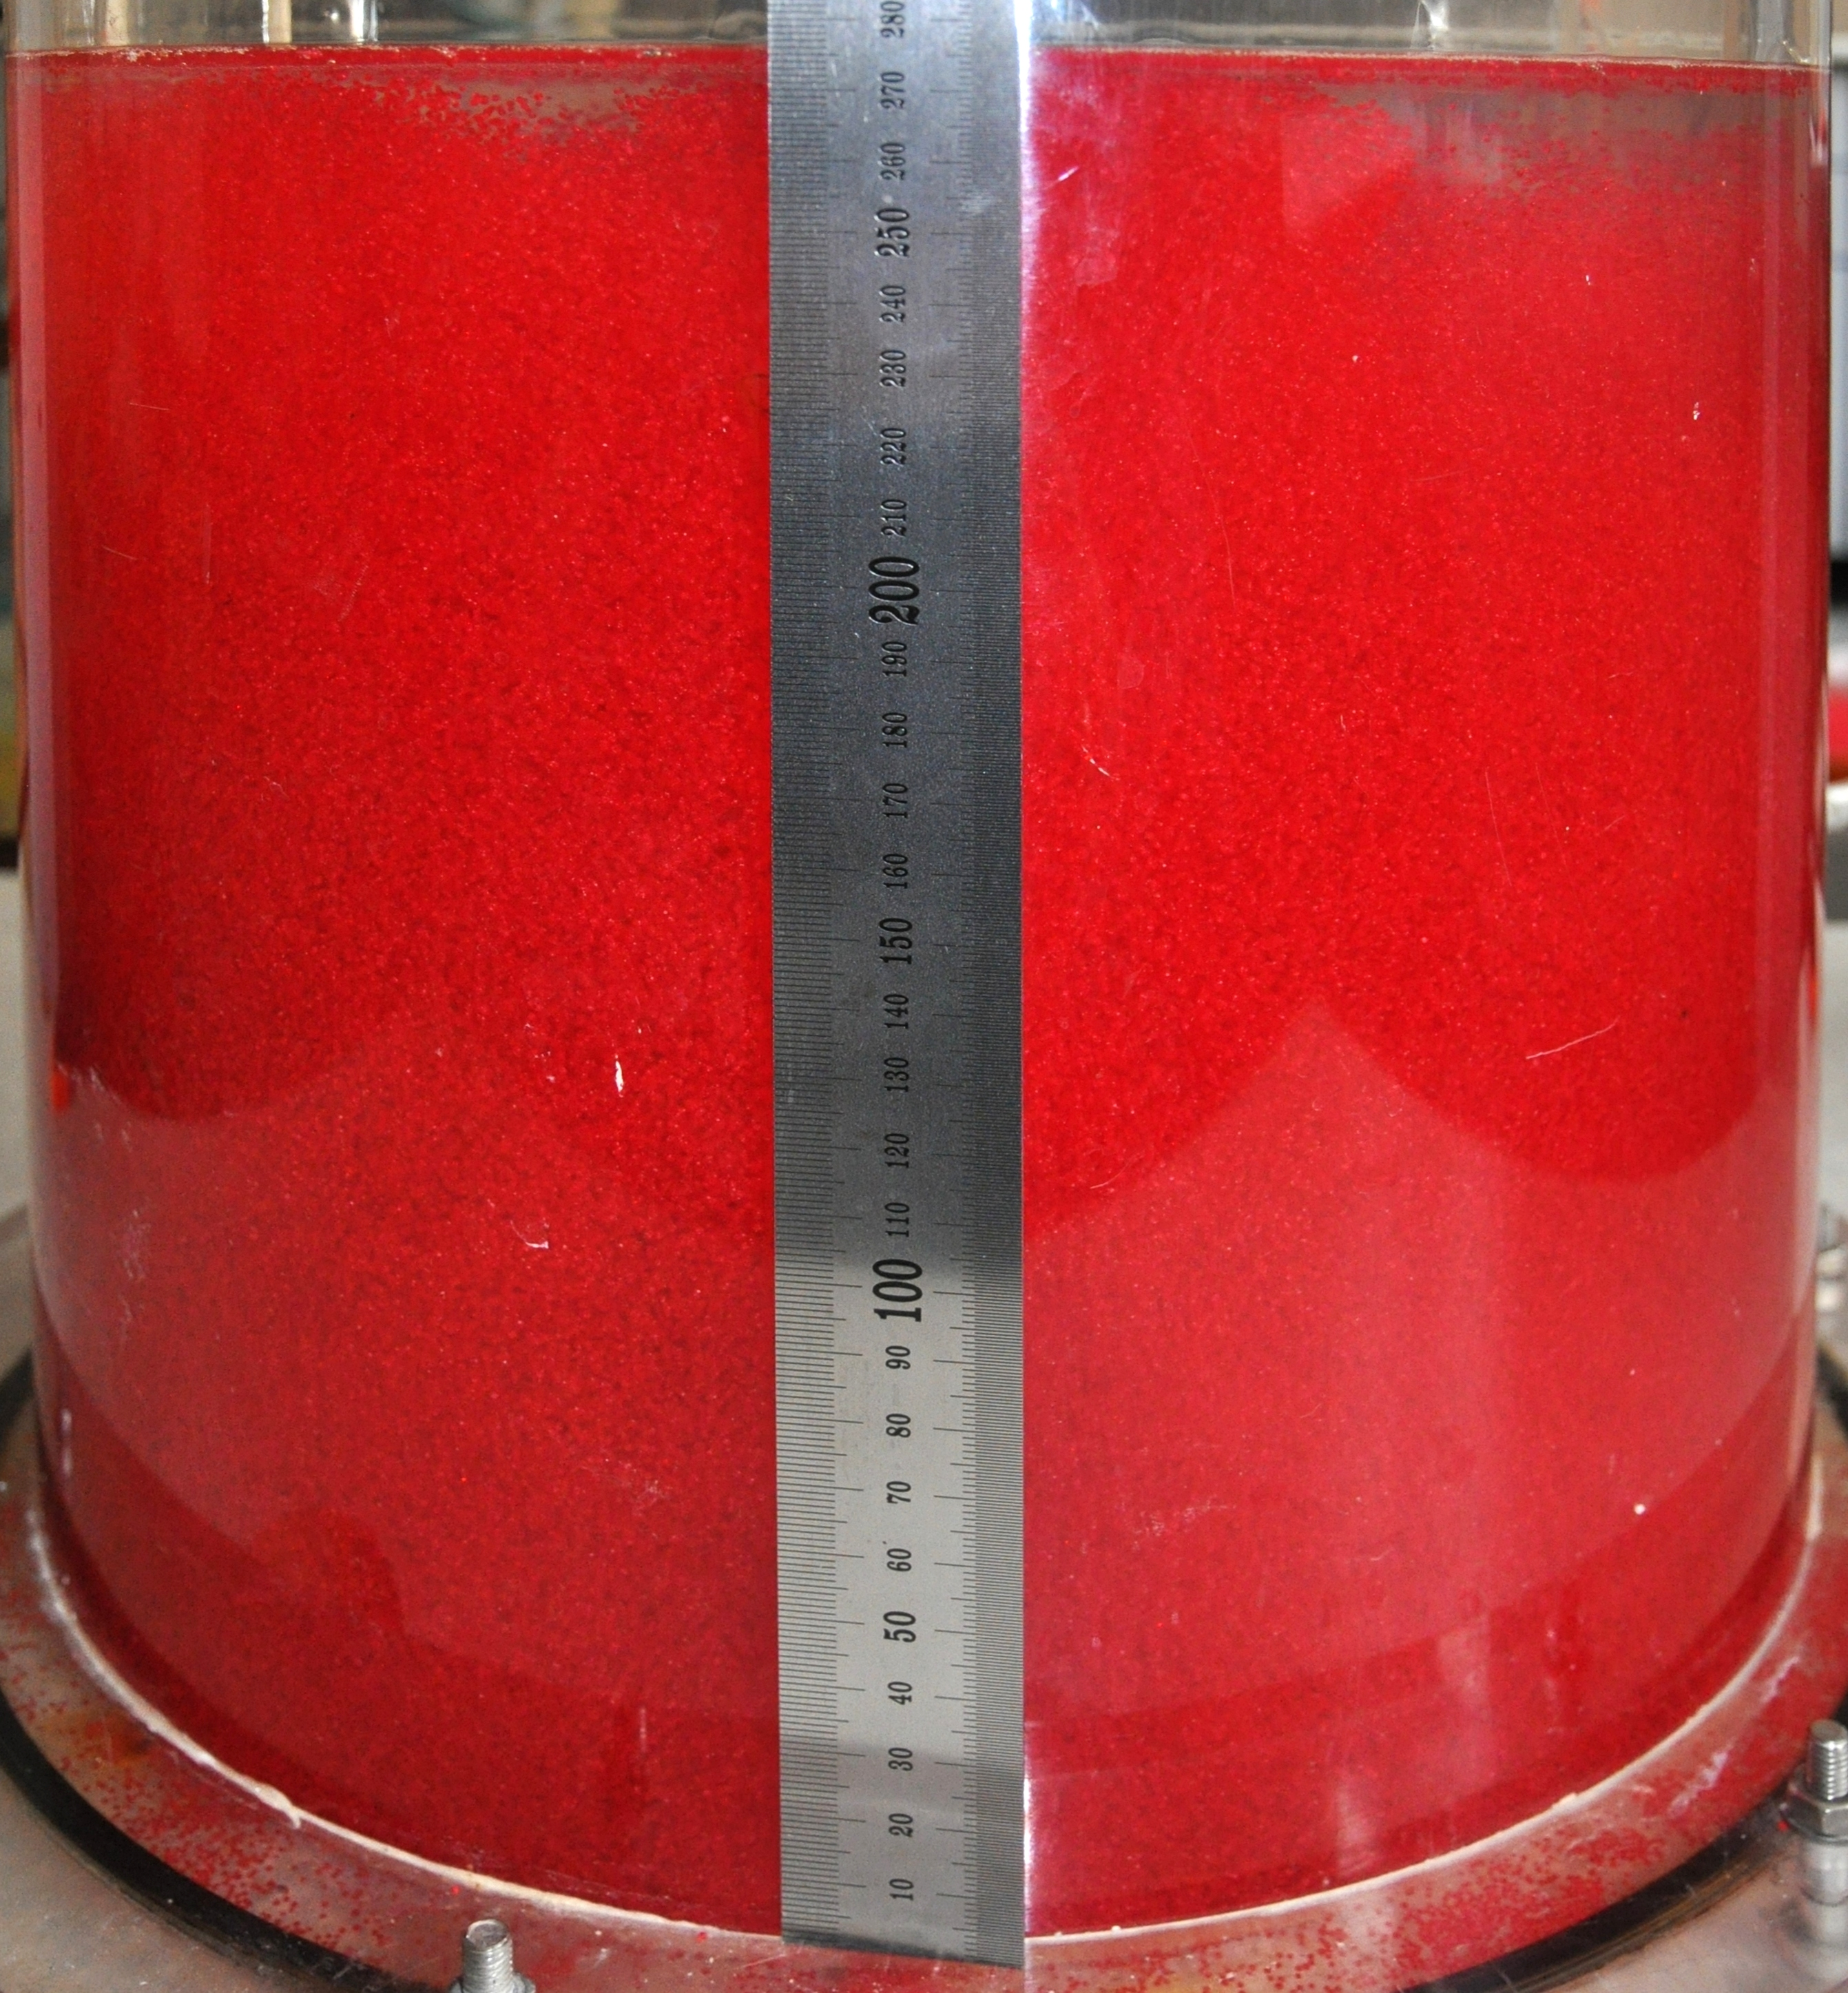
\includegraphics[scale=0.305]{Results/CloudHeight/pvp7-vol10-6s.eps}}
  \caption{Vznos pevné fáze $\kula{N=\SI{6}{\per\second}}$}
  \label{fig:h-w10-6s}
\end{figure}
\newpage

V průběhu nestacionární CFD simulace byla kromě výšky vznosu pevné určována kvalita suspenze ($\sigma$ -- vztah \ref{eq:kvasus}). Získané výsledky pro jednotlivé frekvence otáčení míchadla jsou uvedeny v grafu \ref{grf:qa}. Pro lepší přehlednost jsou tyto závislosti zobrazeny po jedné sekundě simulace. Dle očekávání se čas potřebný k dosažení stavu úplné suspendace s rostoucí rychlostí rotace míchadla zkracoval. V případě $N=\SI{4}{\per\second}$ tato doba přibližně činila \SI{5.7}{\second}, kdežto při $N=\SI{6}{\per\second}$ se zkrátila více než dvojnásobně na zhruba \SI{2.5}{\second}. Navíc v čase kolem \SI{6}{\second} byl zaznamenán přechod do stavu homogenní suspendace pro nejvýše zvolenou frekvenci otáčení míchadla. 

\begin{grf}[h!]
 \centering
  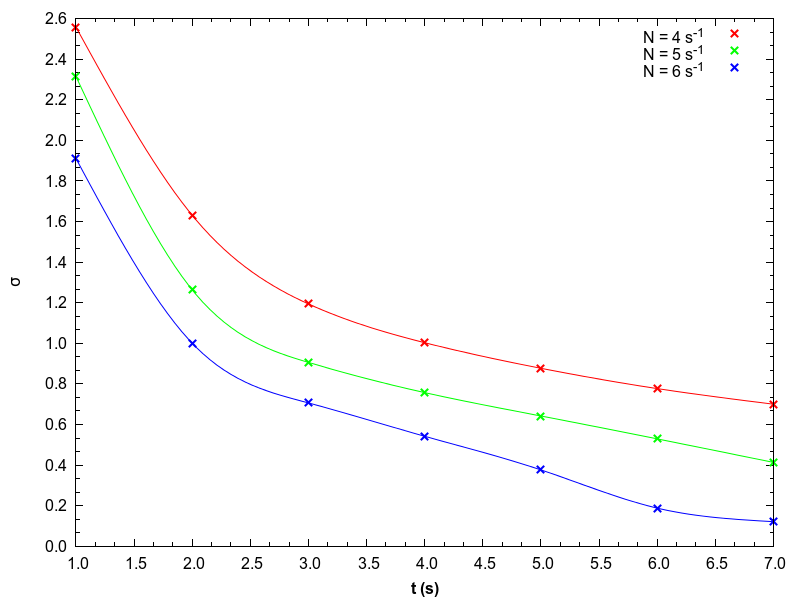
\includegraphics[scale=0.45]{Results/CloudHeight/qa.eps}
  \caption{Průběh kvality suspenze}
  \label{grf:qa}
\end{grf}

\subsection{Srovnání modelů Eulerian-Eulerian a Eulerian-Granular}

\section{Doba homogenizace}
Doba homogenizace v daných systémech byla vyhodnocena pomocí techniky CFD s využitím dříve napočítaných rychlostních polí. Během vlastního stanovení byla řešena pouze transportní rovnice stopovací látky, což znatelně snížilo výpočetní náročnost celého procesu. V průběhu simulací byly zaznamenávány okamžité hodnoty koncentrací stopovací látky v závislosti na čase. Z uložených dat byla poté doba homogenizace určena jako čas potřebný k ustálení této koncentrace v rozmezí \SI{\pm 5}{\percent} její rovnovážné hodnoty.

Nasimulovaný průběh homogenizace indikační látky v řezu nádobou je znázorněn na obrázcích \ref{fig:t}. Jednalo se o systém tvořený vodou a pevnou fází o koncentraci \volproc{5}, přičemž frekvence otáčení míchadla činila \SI{6}{\per\second}. Na obr. \ref{fig:t0} je dobře vidět místo, kde došlo k nadávkování stopovací látky.

\begin{figure}[h!]
 \centering

  \subfloat[$t=\SI{0}{\second}$]{\label{fig:t0}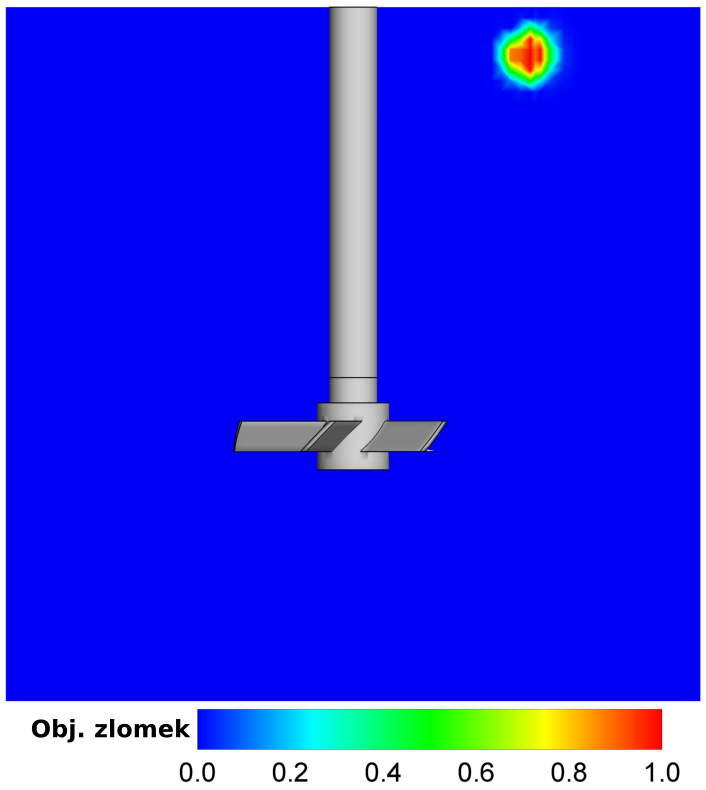
\includegraphics[scale=0.38]{Results/MixingTime/voda-6s/t0.eps}}  
  \qquad             
  \subfloat[{$t=\SI{2}{\second}$}]{\label{fig:t2}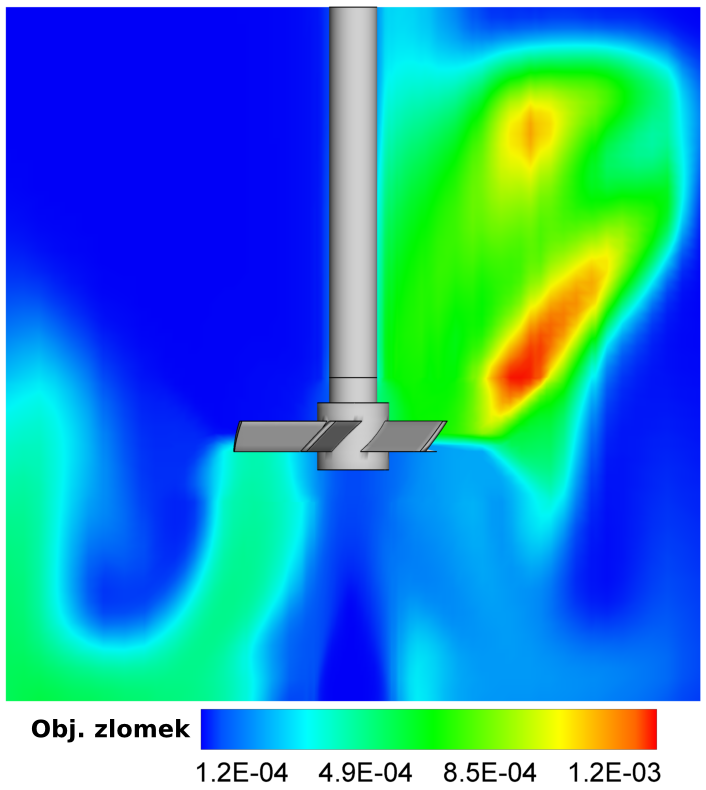
\includegraphics[scale=0.38]{Results/MixingTime/voda-6s/t2.eps}}
  \\
  \subfloat[{$t=\SI{5}{\second}$}]{\label{fig:t5}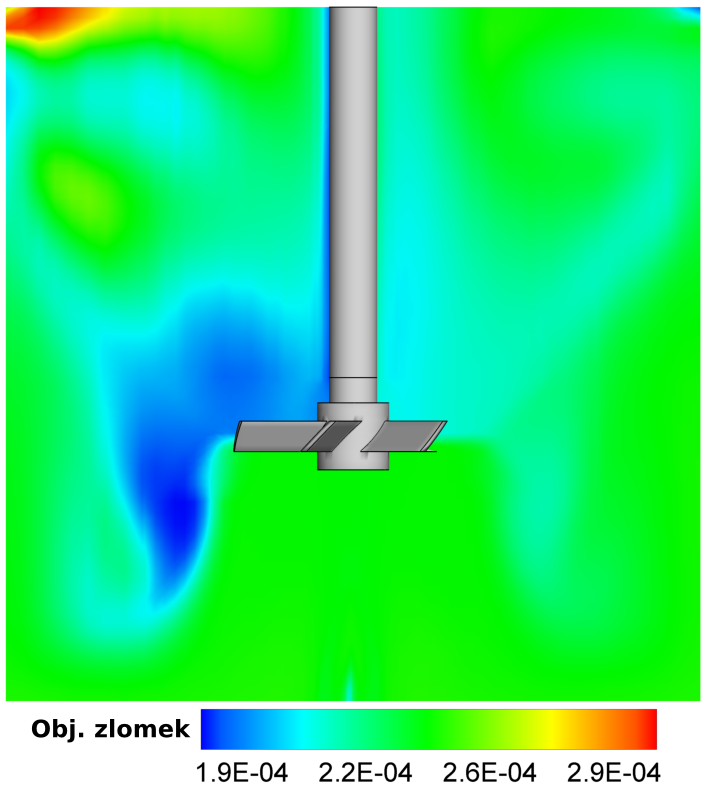
\includegraphics[scale=0.38]{Results/MixingTime/voda-6s/t5.eps}}
  \qquad
  \subfloat[{$t=\SI{7}{\second}$}]{\label{fig:t7}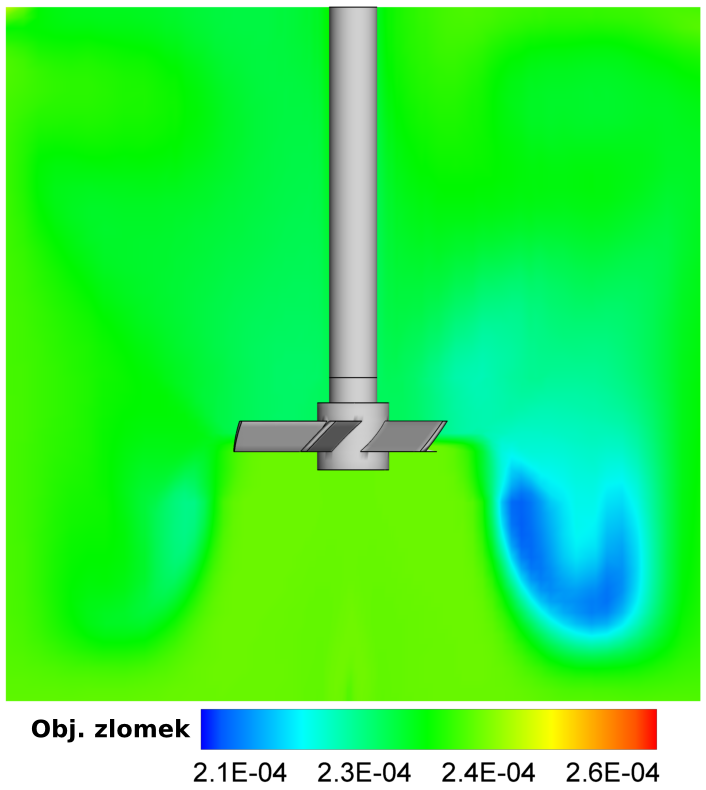
\includegraphics[scale=0.38]{Results/MixingTime/voda-6s/t7.eps}}
  \caption{Koncentrace stopovací látky pro systém voda--PVC \volproc{5} $\kula{N=\SI{6}{\per\second}}$}
  \label{fig:t}
\end{figure}

Následují grafické závislosti bezrozměrné koncentrace stopovací látky na době homogenizace stanovené pomocí techniky CFD. Pro srovnání jsou v grafech vyneseny černou barvou experimentální údaje, které pomocí vodivostní metody stanovila \citet{pav11}. Pro snížení potřebného výpočetního času byly především zkoumány případy s vyšší hodnotou rychlosti rotace míchadla. 

Grafy \ref{fig:homvoda} zachycují výše zmíněné závislosti pro dvoufázový systém reprezentovaný vodou a kuličkami z PVC o koncentraci 5, 10 a \volproc{15} při frekvenci otáčení míchadla \SI{6}{\per\second}. Z vyobrazených průběhů je patrná dobrá shoda mezi experimentálním měřením a výsledky simulací.

\begin{grf}[h!]
 \centering
  \subfloat[\volproc{5} PVC]{\label{fig:homvoda-w5}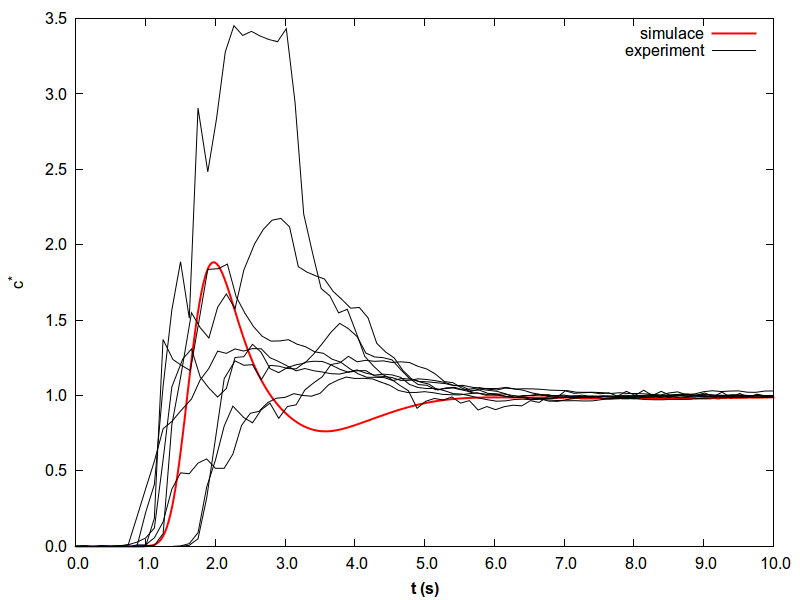
\includegraphics[scale=0.43]{Results/MixingTime/voda-6s/5/grafy.eps}} 
  \\ 
  \subfloat[\volproc{10} PVC]{\label{fig:homvoda-w10}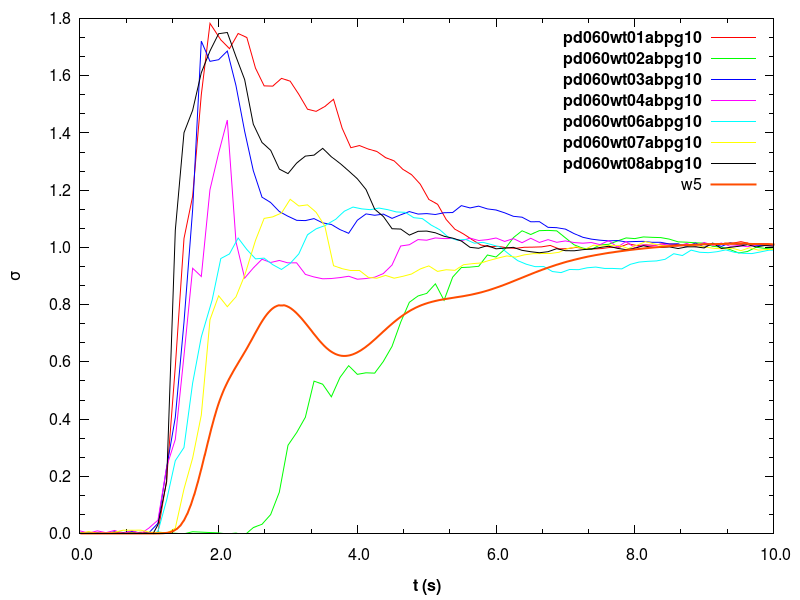
\includegraphics[scale=0.43]{Results/MixingTime/voda-6s/10/grafy.eps}}
\end{grf}
\newpage

\begin{grf}[t!]
  \addtocounter{subgrf}{2}
  \centering
  \subfloat[\volproc{15} PVC]{\label{fig:homvoda-w15}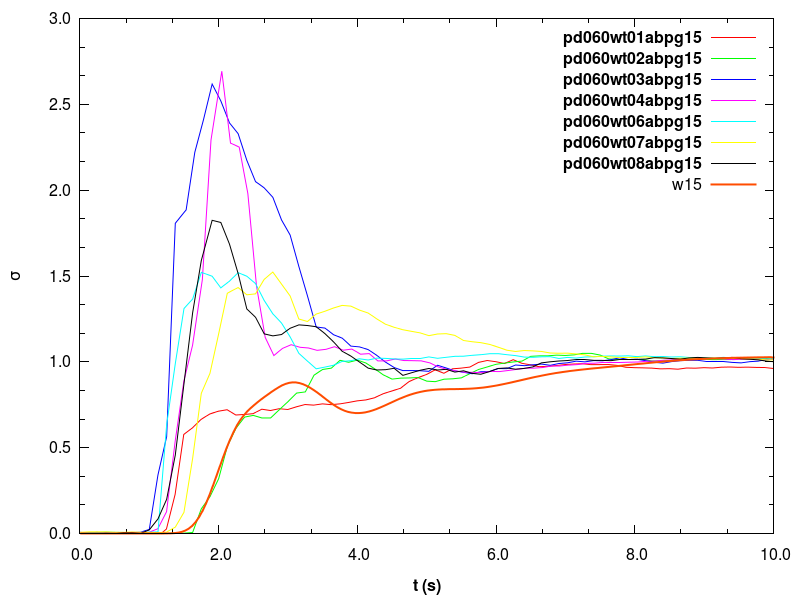
\includegraphics[scale=0.45]{Results/MixingTime/voda-6s/15/grafy.eps}} 
  \caption{Homogenizační křivka pro vodnou suspenzi $\kula{N=\SI{6}{\per\second}}$}
  \label{fig:homvoda}
\end{grf}
\noindent Kromě vodné vsádky byl také simulačně určen průběh bezrozměrné koncentrace indikační látky v čase pro kapalinu \pvpP{} obsahující \volproc{5} pevné fáze. Frekvence otáčení míchadla v tomto případě činila \SI{7}{\per\second}. Získaná závislost je uvedena v grafu \ref{grf:hompvp5}.
\begin{grf}[h!]
 \centering 
  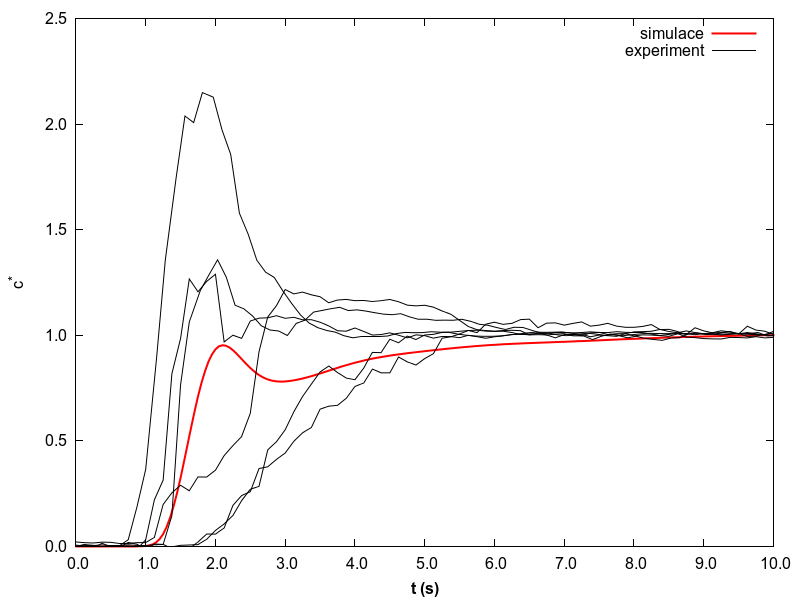
\includegraphics[scale=0.45]{Results/MixingTime/PVP5-7s/5/grafy.eps}
  \caption{Homogenizační křivka pro suspenzi \pvpP{} a \volproc{5} PVC $\kula{N=\SI{7}{\per\second}}$}
  \label{grf:hompvp5}
\end{grf}
\newpage

Tabulka \ref{tab:mixtime} obsahuje hodnoty doby homogenizace pro jednotlivé systémy určené jak pomocí techniky CFD, tak na základě experimentálního měření. Ze simulačních výsledků je vidět, že s rostoucím objemovým zlomkem pevné fáze se taktéž zvyšovala doba homogenizace. Údaje získané pomocí vodivostní metody však tento vzrůstající trend úplně nepotvrdily, neboť nejkratší doba homogenizace byla naměřena pro pevnou fází obsahující \volproc{10} PVC. Kromě vodné vsádky byla také použita kapalina \pvpP{}, jenž díky své vyšší dynamické viskozitě vykazovala delší doby homogenizace v porovnání s vodou. Za zmínku také stojí fakt, že hodnoty doby homogenizace určené pomocí CFD jsou téměř vždy vyšší než experimentálně naměřené. Tento jev je způsoben podhodnocováním turbulentních veličin při použití \keps{} turbulentního modelu.

\begin{table}[h!]
\centering
\caption{Stanovené doby homogenizace v daných systémech}
\label{tab:mixtime}
\begin{tabular}{lcrcc}
\toprule
\textbf{Kapalina} & \textbf{Otáčky} & \textbf{PVC} & \textbf{Experiment} & \textbf{Simulace} \\
\midrule

voda \\
	& \SI{6}{\per\second} & \volproc{5}  & \SI{5.4}{\second} & \SI{5.0}{\second} \\
	& \SI{6}{\per\second} & \volproc{10} &  \SI{5.9}{\second} & \SI{7.2}{\second} \\
	& \SI{6}{\per\second} & \volproc{15} & \SI{5.6}{\second} & \SI{7.7}{\second} \\
\pvpP \\
	& \SI{7}{\per\second} & \volproc{5} & \SI{5.2}{\second} & \SI{5.7}{\second} \\

\bottomrule
\end{tabular}
\end{table}